\documentclass[a4paper, oneside, 12pt]{memoir}

\usepackage{kotex}
\usepackage{amsmath,amssymb,textcomp}
\usepackage{bm}
\usepackage{graphicx}
\usepackage{verbatim}
\usepackage{float}

\newcommand{\bdel}{\bm{\nabla}}
\newcommand{\rd}{\partial}

\setlength{\marginparwidth}{0.1pt}
\setlength{\marginparpush}{0.1pt}
\setlength{\textheight}{0.72\paperheight}
\setlength{\textwidth}{0.8\paperwidth}
\setlength{\uppermargin}{0.15\paperwidth}
\setlength{\spinemargin}{0.15\paperwidth}
\setlength{\marginparsep}{0.15\paperwidth}
\setlength{\oddsidemargin}{-12pt}
\setlength{\evensidemargin}{-12pt}

\setsecnumdepth{subsection}
\maxtocdepth{subsection}

\usepackage{color}
\usepackage{listings}
\definecolor{Brown}{cmyk}{0,0.81,1,0.60}
\definecolor{OliveGreen}{cmyk}{0.64,0,0.95,0.40}
\definecolor{CadetBlue}{cmyk}{0.62,0.57,0.23,0}
\lstset{language=C++,frame=ltrb,framesep=5pt,basicstyle=\scriptsize,
keywordstyle=\ttfamily\color{OliveGreen},
identifierstyle=\ttfamily\color{CadetBlue}\bfseries,
commentstyle=\color{Brown},
stringstyle=\ttfamily,
showstringspaces=false}

\newfloat{code}{bth}{loc}
\floatname{code}{Code}
\renewcommand{\thecode}{\arabic{chapter}.\arabic{code}}

\newenvironment{pc}
{
\\
\noindent
\begin{minipage}[c]{\textwidth}
}
{
\end{minipage}
\\
}

\title{GEANT4 무작정 따라하기}
\author{장 진희\\geniejhang@majimak.com}

\begin{document}
\maketitle
\begin{center}
Second Edition

Based on the advice of \textbf{Kisoo Lee}
\end{center}
\thispagestyle{empty}

\newpage
\tableofcontents
\listof{code}{List of Codes}

\newpage
\chapter{간단한 소개}
아직 아는것이 많지 않기에, 아는것이 생긴다면 시간이 되는대로 업데이트
하겠다. 일단은 지금까지 시행착오도 많이 거치며 알아낸 것들을 정리하기 위해서 이
문서를 쓴다. 나중에 어떻게 될지는 모르겠지만, 가능한 나보다 늦게 시뮬레이션을
시작하는 사람이 나보다 적은 시간을 들여 내가 알아낸 것들을 알 수 있도록 쓸
것이다.

\vspace{5mm}
GEANT는 Geometry ANd Tracking의 약자로, 뒤에있는 4는 당연히 4번째
버전임을 나타낸다. GEANT4는 컴퓨터 안에서 가상의 실험실을 만들고, 그 안에 여러
검출기를 놓아두고 빔(입자 혹은 광자)을 이용해서 실험하는 것을 도와주는
\emph{Library Package}이다. 우리가 해야할 것은 이 패키지에서 적절한 것을 꺼내와
적절하게 배치하고, 실행시켜주는것이다.

라이브러리 패키지가 뭔지 잘 다가오지 않는 나같은 사람이 있을지도 몰라 간단히
설명해보도록 하겠다. 아무것도 없는 상태에서 시뮬레이션을 하려고 한다고 해보자.
먼저 기본 단위를 정해야 한다. 길이, 시간, 에너지, 전하량 등등. 계산을 좀 편하게
하기 위해서, 숫자 세개의 묶음이 벡터라는것도 알려줘야 하고, 이 벡터들 사이에
연산 방법을 알려줘야 한다. 속도를 알려주면, 이 속도라는게 정해준 단위 시간당
얼마만큼의 거리를 프로그램내에서 진행한다는 것을 알려줘야 한다. 검출기나 기타
물질들과 어떤 상호작용을 하는지 알려줘야 한다. 이처럼 여러가지 해야할 것들을
하나의 패키지로 묶어서 사용할 수 있게 해놓은것이 라이브러리 패키지이다.

\vspace{5mm}
\emph{참고}: 이 문서는 GEANT4.9.4.p01버전과 CLHEP\_2.1.0.1버전을 이용해서
만들어졌다. 나중에 GEANT4가 업데이트 되면서 실행이 안되는 부분이 생길 수도
있다.

\chapter{최종 결과 \label{chapter-2}}

이 문서를 다 읽고, 그대로 다 따라한 후에 얻어낸 결과는 이렇다.

\begin{figure}[h]
\centering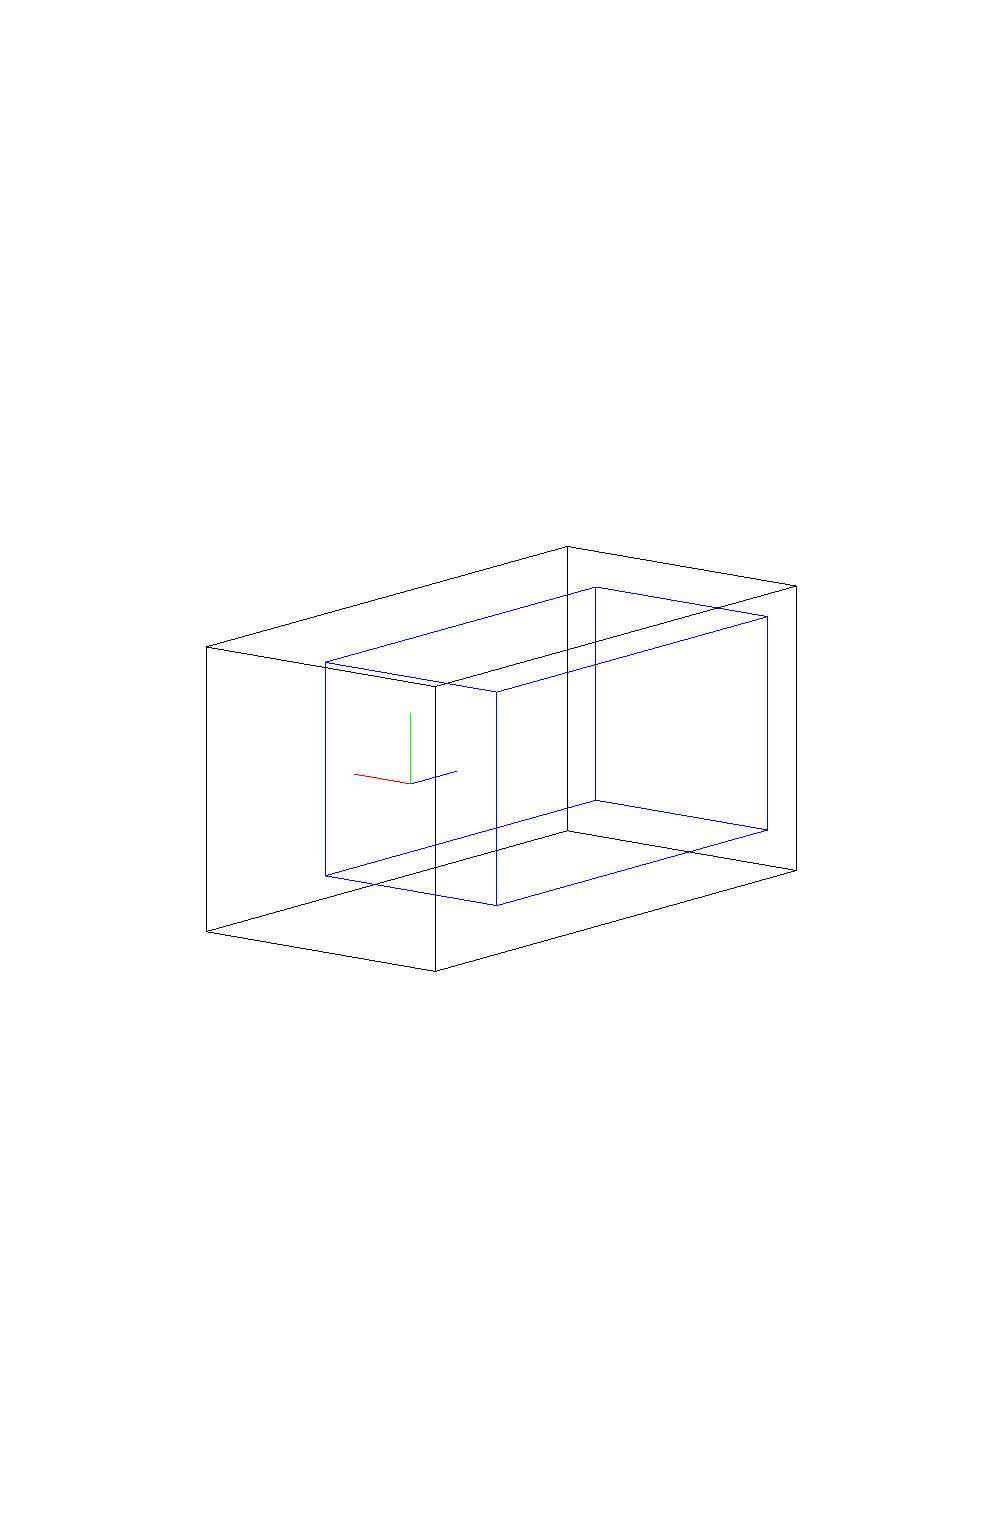
\includegraphics[width=0.5\textwidth]{tex/tiltview.pdf}
\centering\caption{실험실 전체를 비스듬히 본 그림. RGB순으로 $xyz$축이다.}
\end{figure}

\begin{figure}[h]
\centering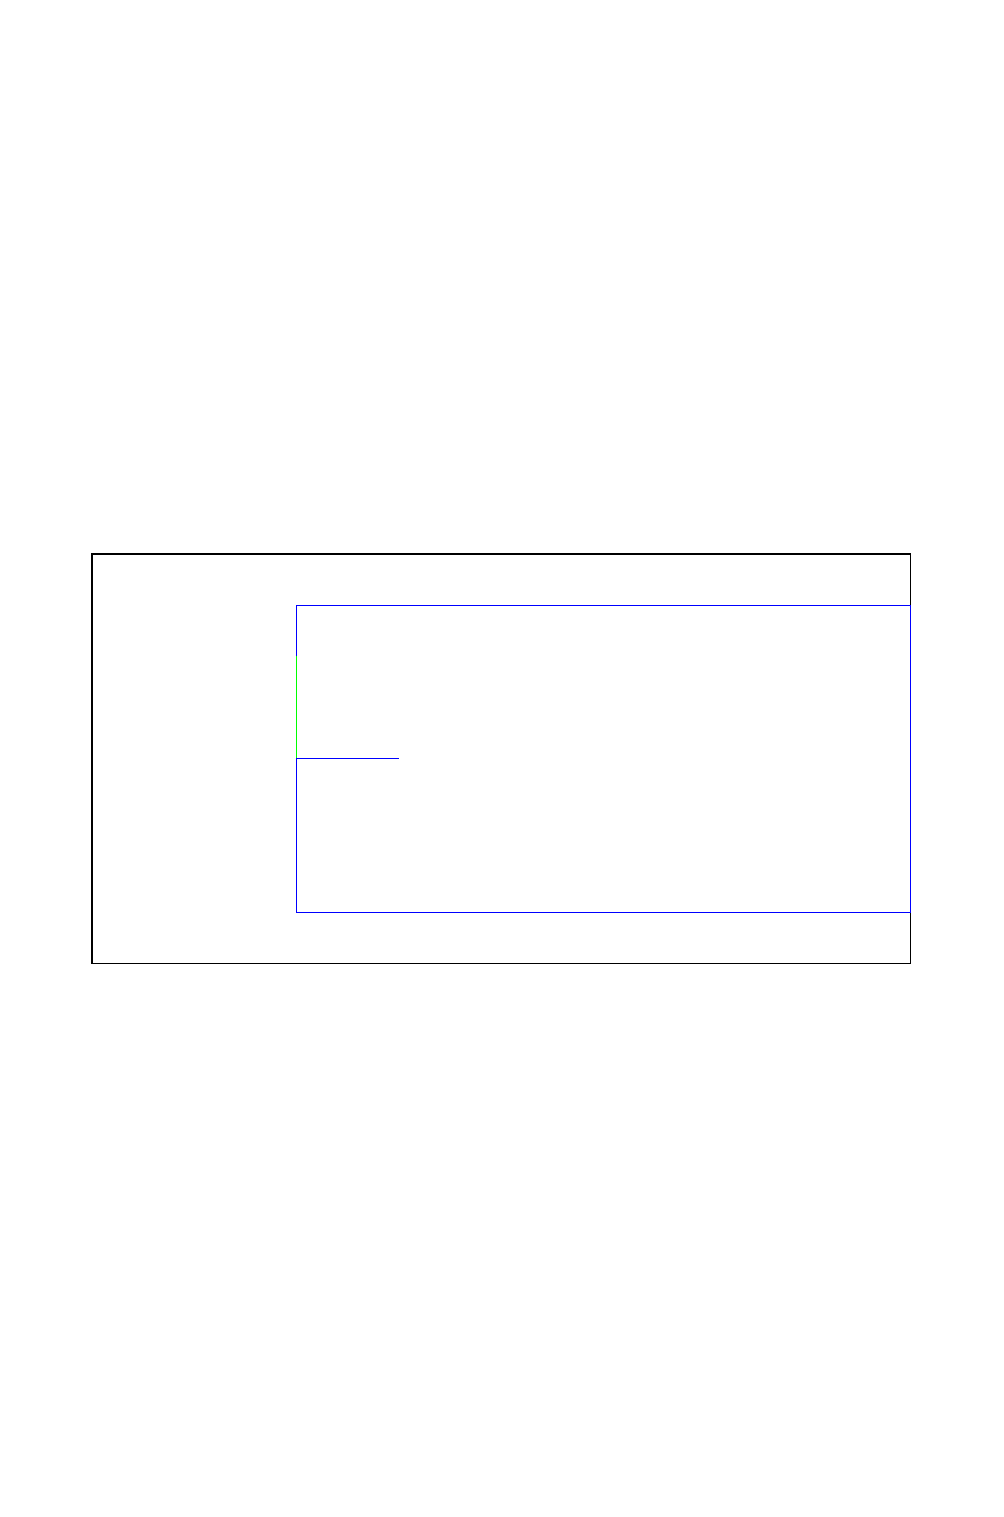
\includegraphics[width=0.5\textwidth]{tex/sideview.pdf}
\centering\caption{실험실 전체를 옆에서 본 그림.}
\end{figure}

실험실 크기는 $20\times20\times40$ cm이고, 검출기로 사용할 Scintillator는
$15\times15\times30$ cm이며, $10\times10\times1$ mm의 작은 조각별로 저장된
에너지를 읽을 수 있다고 가정한다. 이 Scintillator Array의 중심은 $(0, 0, 5
\text{ cm})$에 위치돼 있다. 입사하는 빔은 150 MeV의 양성자 빔을 사용할 것이고,
Scintillator의 바로 앞인 $(0, 0, -10 \text{ cm})$에서 쏠 것이다.

10000개의 양성자를 이러한 구조의 Scintillator에 쏘아서 나온 데이타를 가지고
그래프를 그려보면 그림~\eqref{finalResult}과 같은 결과를 얻을
수 있다.

\begin{figure}[h]
\centering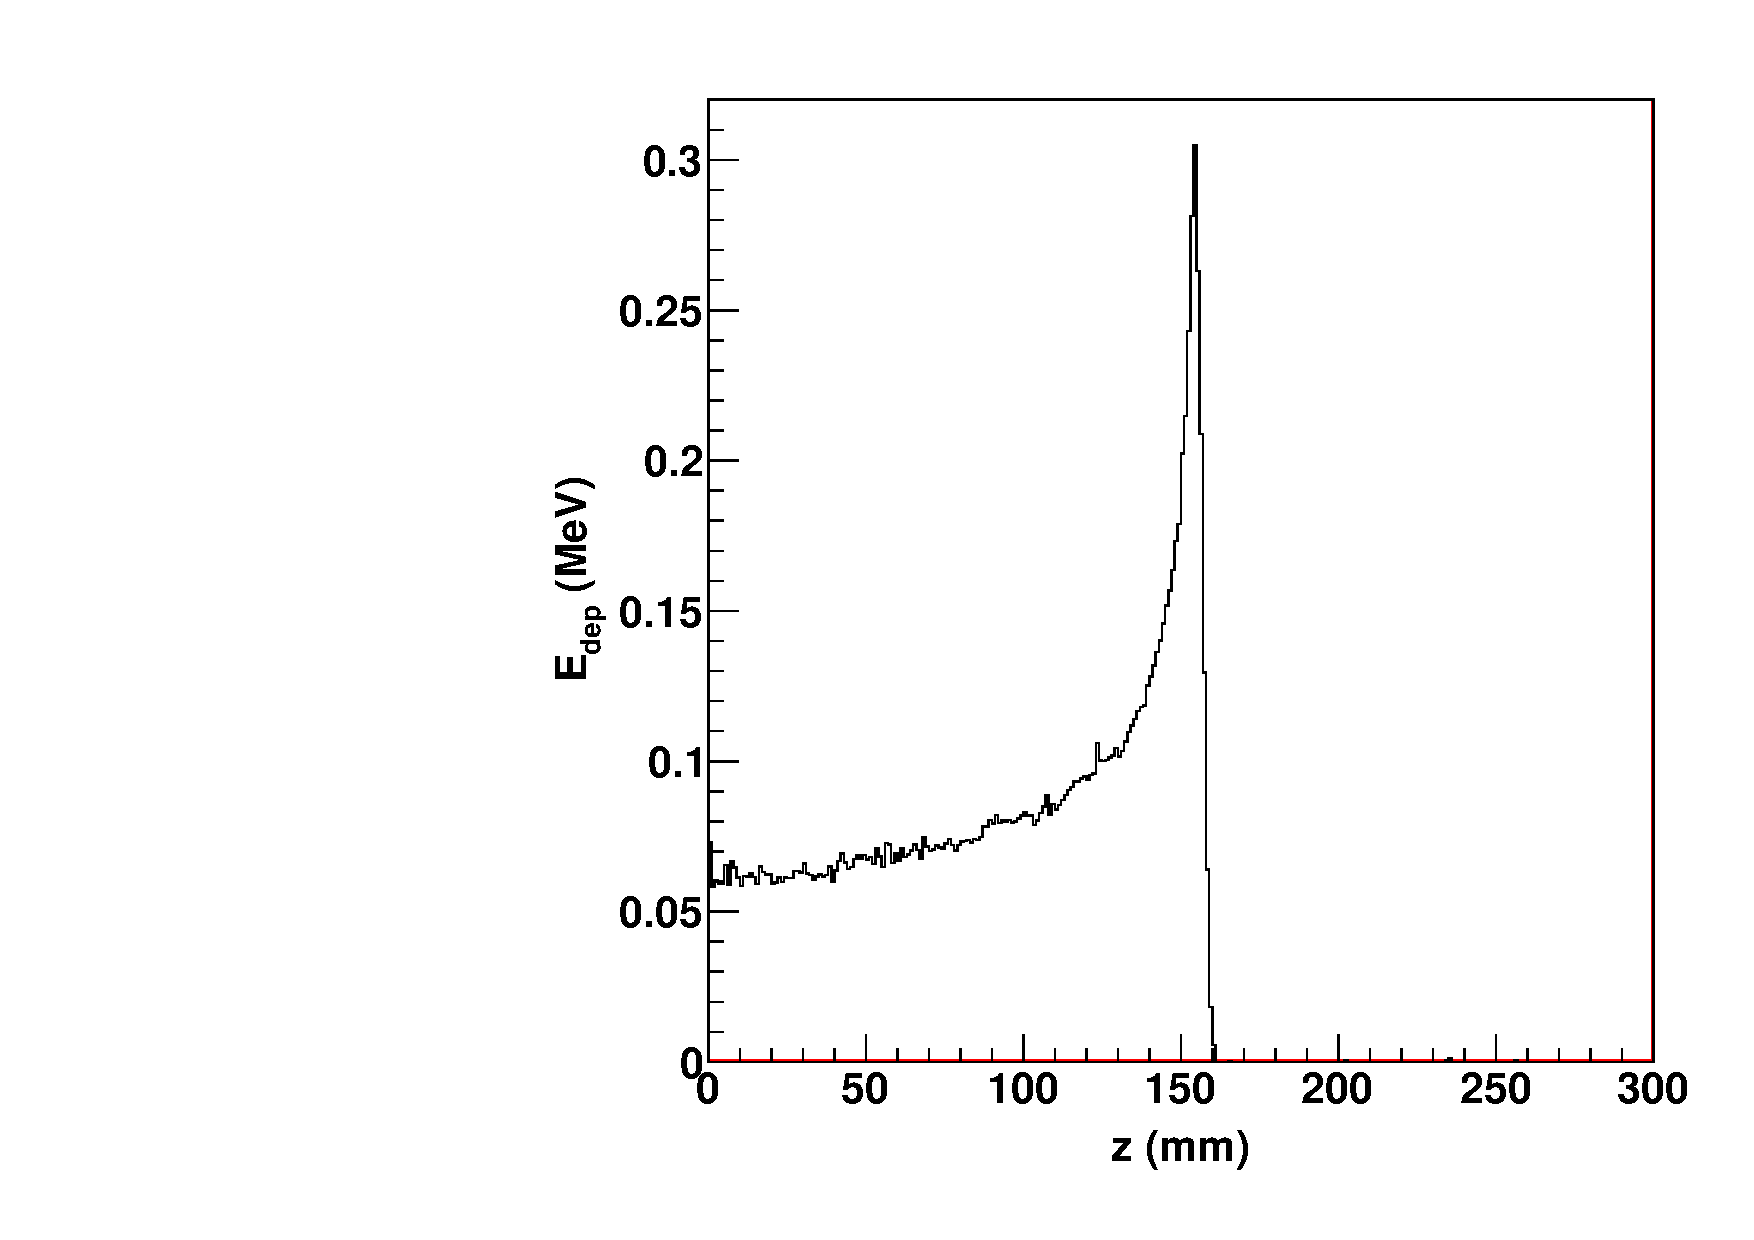
\includegraphics[width=0.7\textwidth]{tex/finalResult.pdf}
\centering\caption{양성자에 의한 Bragg Peak \label{finalResult}}
\end{figure}

\chapter{해보자!}

일단 간단하게 이것저것에 대해 알아보자. 예제 시뮬레이션의 이름은
\texttt{example}이라고 하자.

\section{가장 기본적인 파일들}

시뮬레이션을 하기위한 가장 기본적인 파일구조는 아래와 같다.
\begin{verbatim}
- main directory
  - GNUmakefile
  - example.cc
    - "include" directory
      - examplePhysicsList.hh
      - exampleDetectorConstruction.hh
      - examplePrimaryGeneratorAction.hh
    - "src" directory
      - examplePhysicsList.cc
      - exampleDetectorConstruction.cc
      - examplePrimaryGeneratorAction.cc
\end{verbatim}
사실 파일명은 아무렇게나 적어줘도, \texttt{example.cc}파일에서 각 기능을 할당할 때
제대로만 할당해주면 시뮬레이션 자체에는 무리가 없다. 하지만, 그렇게 했을 때
다른사람은 물론이거니와 코드를 짠 본인조차도 뭘했는지 한참을 생각해야 하는
사태가 발생하니 이대로 하도록 하자. 또, 이 문서에 나와있는 파일명들은
GEANT4 설치 디렉토리에 있는 예제들에 맞췄기 때문에, 여기서 설명하는것을 잘
이해해 둔다면 예제들을 이해하는 시간을 단축시킬 수 있으리라 본다.

\subsection{GNUmakefile}
이 파일은 \texttt{make}라는 명령어를 이용해서 코드 전체를 쉽게 컴파일하고 실행파일로
만드는 것을 도와준다. 파일 내용은 아래와 같다.

\begin{code}[h]
\begin{lstlisting}
1 name      := example
2 G4TARGET  := $(name)
3 G4EXLIB   := true
4 G4WORKDIR := ./
5 
6 .PHONY: all
7 all: lib bin
8 
9 include $(G4INSTALL)/config/binmake.gmk
\end{lstlisting}
\caption{\texttt{GNUmakefile} (Complete without using ROOT) \label{code-3-1}}
\end{code}
한번 만들어놓으면 \texttt{name}이외에는 바꿀일이 거의 없으므로 그냥 가져다 쓰도록
하자.

\vspace{5mm}
\emph{참고}: 나중에 시뮬레이션에서 나오는 값들을 ROOT형태로 출력하려면 이
파일에 ROOT 라이브러리에 관한 정보를 줘야 한다. 쓰고는 있지만, 아직 확실히
모르겠으므로 동작하는 파일을 붙여넣기만 하겠다. Code~\ref{code-3-1-5}에 있다.

\begin{code}[h]
\begin{lstlisting}
  1 name := LAMPS_Output
  2 G4TARGET := $(name)
  3 G4EXLIB := true
  4 G4WORKDIR := ./
  5 
  6 SOFLAGS        += -shared
  7 ROOTLIBS       := $(shell root-config --libs)
  8 ROOTCFLAGS     := $(shell root-config --cflags)
  9 ROOTGLIBS      := $(shell root-config --glibs)
 10 CXXFLAGS        = -m64 -O -Wall -fPIC 
 11 CXXFLAGS       += $(ROOTCFLAGS) 
 12 CPPFLAGS        = -m64 -O -Wall -fPIC
 13 CPPFLAGS       += $(ROOTCFLAGS) 
 14 
 15 CPPFLAGS += -DG4ANALYSIS_USE_ROOT
 16 CPPFLAGS += -D_REENTRANT -I$(ROOTSYS)/include
 17 
 18 CPPFLAGS += -pthread -I$(ROOTSYS)/include
 19 ROOTLIBS = $(shell $(ROOTSYS)/bin/root-config --nonew --libs)
 20 EXTRALIBS := $(ROOTLIBS)
 21 EXTRALIBS += -L$(ROOTSYS)/lib \
 22 -lCore -lCint \
 23 -lHist -lGraf -lGraf3d -lGpad \
 24 -lTree -lRint -lPostscript \
 25 -lMatrix -lPhysics \
 26 -lm -ldl -lpthread -rdynamic
 27 
 28 #ifndef G4INSTALL
 29 # G4INSTALL = ../
 30 #endif
 31 
 32 #ifndef G4WORKDIR
 33 # G4WORKDIR = .
 34 #endif
 35 
 36 .PHONY: all
 37 all: lib bin
 38 
 39 include $(G4INSTALL)/config/binmake.gmk
\end{lstlisting}
\caption{\texttt{GNUmakefile} (Complete with using ROOT) \label{code-3-1-5}}
\end{code}

\newpage
\subsection{PhysicsList}
시뮬레이션에서 사용할 입자들을 등록하고, 상호작용에 사용할 모델들을 등록한다.
당장은 특별한 시뮬레이션을 하는것이 아니므로, 모든 것이 다 들어있다는
\texttt{A01PhysicsList}를 가져다 사용하도록 하자. \texttt{A01PhysicsList}는
\begin{pc}
\begin{lstlisting}
$G4INSTALL/examples/extended/analysis/A01/
\end{lstlisting}
\end{pc}
에 있고, 필요한 파일들은 아래와 같다.

\begin{verbatim}
- "include" directory
  - A01PhysicsList.hh
  - A01GeneralPhysics.hh
  - A01MuonPhysics.hh
  - A01EMPhysics.hh
  - A01HadronPhysics.hh
  - A01IonPhysics.hh
- "src" directory
  - A01PhysicsList.cc
  - A01GeneralPhysics.cc
  - A01MuonPhysics.cc
  - A01EMPhysics.cc
  - A01HadronPhysics.cc
  - A01IonPhysics.cc
\end{verbatim}

위 파일들을 복사해 와서 \texttt{include}디렉토리와 \texttt{src}디렉토리에 잘
넣어준다. 한가지 고칠 것이 있는데, \texttt{src}디렉토리 안에
\texttt{A01PhysicsList.cc}파일을 열어 74번째 줄에
\begin{pc}
\begin{lstlisting}
74   defaultCutValue = 1.0*mm;
\end{lstlisting}
\end{pc}
를 찾아 아래와 같이 고쳐준다.
\begin{pc}
\begin{lstlisting}
74   defaultCutValue = 10.0*um;
\end{lstlisting}
\end{pc}
``Geant4 User's Guide for Application Developers''에 보면, 이 컷에 대한 설명이
이렇게 나와있다.
\begin{quote}
This range cut value is converted threshold energies for each material and for
each particle type (i.e. electron, positron and gamma) so that the particle
with threshold energy stops (or is absorbed) after traveling the range cut
distance.
\end{quote}
간단히 말하면 컷 값이 크면 한 스텝이 길고, 작으면 스텔 길이가 짧다는 소리다.
컷값을 매우 작게하면 시뮬레이션은 정확해지겠지만 시간이 무한정 길어지고, 컷값을
너무 크게 하면 시뮬레이션은 빨라지지만 부정확한 결과가 나온다. 보고자 하는
결과와 검출기의 구조에 맞춰서 적절한 컷값을 주면 빠르고 정확한 결과를 얻어낼 수
있다.

\subsection{DetectorConstruction}
GEANT4 예제 대부분의 소스코드들은 파일명으로 그 코드가 뭘 하는지 알려준다.
파일명에서 알 수 있듯이 컴퓨터 안에 검출기를 만들어주는 부분이다. 파일명이
이렇다고 컴퓨터가 다 알아서 해주는것은 아니고 자기가 코드는 다 짜야한다.
헤더파일(\texttt{.hh})과 소스파일(\texttt{.cc})의 기본적인 뼈대는
Code~\ref{code-3-2}과~\ref{code-3-3}와 같다. 헤더파일의 15번째 줄을 보면,
\begin{pc}
\begin{lstlisting}
 15     virtual G4VPhysicalVolume* Construct();
\end{lstlisting}
\end{pc}
이렇게 돼 있다. GEANT4 시뮬레이션 프로그램을 다 짠 후 실행을 시키면 프로그램이
알아서 \texttt{G4VPhysicalVolume} 형식의 주소를 반환하는 \texttt{Construct()}함수를
실행시켜서 메모리상에 사용자가 만든 구조대로 검출기를 만드는 일을 한다.
그렇기 때문에 없어서는 안될 함수이다.
\begin{pc}
\begin{lstlisting}
 20     void DefineDimensions();
 25     void ConstructMaterials();
 26     void DestructMaterials();
\end{lstlisting}
\end{pc}
이 세 줄의 함수는 기본구조에는 포함되지 않지만, 나아아아아중에 혹시 메신저라는
방법을 이용해서 사용자와 상호작용할 수 있는 검출기를 시뮬레이션 할 때
필요할지도 모르니 넣어둔다. 함수 이름에서 알 수 있듯이 검출기의 치수들을
정의하고, 검출기에 사용할 물질을 만드는 역할과 시뮬레이션이 다 끝난 후
만들어놨던 물질들을 없애는 역할을 한다. 여기서 만들고 없앤다는것은 메모리
상에서의 이야기이다. Detector Construction의 소스코드~\ref{code-3-3}를 보면, 이
클래스의 생성자에 \texttt{ConstructMaterials()}함수와
\texttt{DefineDimensions()}함수가 들어가 있고, 소멸자에
\texttt{DestructMaterials()}함수가 들어가 있는것을 볼 수 있다. 이게 바로
방금 말했던 이야기다. 코드들을 복사해서 각 파일로 만들어 알맞는 디렉토리에
넣어준다. 

\begin{code}[p]
\begin{lstlisting}
  1 #ifndef exampleDetectorConstruction_h
  2 #define exampleDetectorConstruction_h 1
  3 
  4 #include "globals.hh"
  5 #include "G4VUserDetectorConstruction.hh"
  6 
  7 class G4VPhysicalVolume;
  8 
  9 class exampleDetectorConstruction: public G4VUserDetectorConstruction
 10 {
 11   public:
 12     exampleDetectorConstruction();
 13     virtual ~exampleDetectorConstruction();
 14 
 15     virtual G4VPhysicalVolume* Construct();
 16 
 17   private:
 18     // comment: When you change dimensions of a detector in the interactive
 19     //          mode, dimensions should be set outside of Construct().
 20     void DefineDimensions();
 21 
 22     // comment: You'd better define all material pointers here and initialize
 23     //          them as 0 in the constructor. Finally, allocate them in
 24     //          function below.
 25     void ConstructMaterials();
 26     void DestructMaterials();
 27 };
 28 #endif
\end{lstlisting}
\caption{\texttt{exampleDetectorConstruction.hh} (Skeleton) \label{code-3-2}}
\end{code}

\begin{code}[p]
\begin{lstlisting}
  1 #include "exampleDetectorConstruction.hh"
  2 
  3 #include "G4LogicalVolume.hh"
  4 #include "G4VPhysicalVolume.hh"
  5 
  6 exampleDetectorConstruction::exampleDetectorConstruction()
  7 {
  8   ConstructMaterials();
  9   DefineDimensions();
 10 }
 11 
 12 exampleDetectorConstruction::~exampleDetectorConstruction()
 13 {
 14   DestructMaterials();
 15 }
 16 
 17 exampleDetectorConstruction::DefineDimensions()
 18 {
 19 }
 20 
 21 G4VPhysicalVolume* exampleDetectorConstruction::Construct()
 22 {
 23 }
 24 
 25 void exampleDetectorConstruction::ConstructMaterials()
 26 {
 27 }
 28 
 29 void exampleDetectorConstruction::DestructMaterials()
 30 {
 31 }
\end{lstlisting}
\caption{\texttt{exampleDetectorConstruction.cc} (Skeleton) \label{code-3-3}}
\end{code}

\newpage
\newpage
\subsection{PrimaryGeneratorAction}

이름을 이용해서 뭘하는지 유추해보자면, Primary (vertex)의 Generator가 하는
Action을 정의해주는 곳이다. 이 파일에서는 빔으로 어떤 입자를 이용할 것인지,
처음 빔이 나오는 곳은 어디인지, 어느 방향으로 얼마만큼의 에너지를 가지고 빔이
나가는지 등 빔에 대한 것들을 정할 수 있다. 가장 기본적인 구조는
Code~\ref{code-3-4}과~\ref{code-3-5}에 나와 있다. Code~\ref{code-3-4}에 보면
\begin{pc}
\begin{lstlisting}
 17     virtual void GeneratePrimaries(G4Event* anEvent);
\end{lstlisting}
\end{pc}
라는 줄이 있는데, 이것 역시 프로그램이 알아서 \texttt{G4Event}형식의 포인터를
이 함수로 넘겨주어 그 이벤트에 해당하는 빔을 만들도록 자동으로 지시하므로
없으면 에러를 보내온다. 여기서도 역시, 기본적인 구조로 파일을 일단 만들어 놓는다.

\begin{code}[p]
\begin{lstlisting}
  1 #ifndef examplePrimaryGeneratorAction_h
  2 #define examplePrimaryGeneratorAction_h 1
  3 
  4 #include "G4VUserPrimaryGeneratorAction.hh"
  5 
  6 class G4ParticleGun;
  7 
  8 class examplePrimaryGeneratorAction: public G4VUserPrimaryGeneratorAction
  9 {
 10   private:
 11     G4ParticleGun* particleGun;
 12 
 13   public:
 14     examplePrimaryGeneratorAction();
 15     ~examplePrimaryGeneratorAction();
 16 
 17     virtual void GeneratePrimaries(G4Event* anEvent);
 18 };
 19 #endif
\end{lstlisting}
\caption{\texttt{examplePrimaryGeneratorAction.hh} (Skeleton) \label{code-3-4}}
\end{code}

\begin{code}[p]
\begin{lstlisting}
  1 #include "examplePrimaryGeneratorAction.hh"
  2 
  3 #include "G4ParticleGun.hh"
  4 #include "G4Event.hh"
  5 #include "G4IonTable.hh"
  6 #include "G4UnitsTable.hh"
  7 #include "G4ThreeVector.hh"
  8 #include "G4ParticleDefinition.hh"
  9 
 10 examplePrimaryGeneratorAction::examplePrimaryGeneratorAction()
 11 {
 12   particleGun = new G4ParticleGun;
 13 }
 14 
 15 examplePrimaryGeneratorAction::~examplePrimaryGeneratorAction()
 16 {
 17   delete particleGun;
 18 }
 19 
 20 void examplePrimaryGeneratorAction::GeneratePrimaries(G4Event* anEvent)
 21 {
 22 }
\end{lstlisting}
\caption{\texttt{examplePrimaryGeneratorAction.cc} (Skeleton) \label{code-3-5}}
\end{code}

\subsection{example.cc}

이제 가장 중요한 것이 남았다! 지금까지 만든 파일들을 연결을 해줘야 한다.
GEANT라이브러리를 불러와서 시뮬레이션 프로그램을 만들고, 검출기 구조와 빔
정보가 들어가 있는 파일이 어느것인지 알려주고 시뮬레이션을 시작해줄 구동파일이
필요하다. 파일의 소스코드는 Code~\ref{code-3-6}에 있다.

이 코드는 좀 설명이 필요하다.
\begin{pc}
\begin{lstlisting}
  1 #include "G4RunManager.hh"
  2 #include "A01PhysicsList.hh"
  3 #include "exampleDetectorConstruction.hh"
  4 #include "examplePrimaryGeneratorAction.hh"
\end{lstlisting}
\end{pc}
순서대로 \texttt{G4RunManager}, \texttt{A01PhysicsList},
\texttt{exampleDetectorConstruction} 그리고 \\
\texttt{examplePrimaryGeneratorAction}의 헤더파일을 불러와 사용할 준비를 한다.
이렇게만 써놓으면 GEANT4의 설치 경로에 있는 헤더파일들이 있는 디렉토리와 유저가 만든
헤더파일 디렉토리를 알아서 검색해서 찾아낸다.
\begin{pc}
\begin{lstlisting}
  8   G4RunManager *runManager = new G4RunManager();
\end{lstlisting}
\end{pc}
\texttt{G4RunManager}를 불러오고,
\begin{pc}
\begin{lstlisting}
 10   exampleDetectorConstruction* exampleDC = new exampleDetectorConstruction();
 11   runManager -> SetUserInitialization(exampleDC);
\end{lstlisting}
\end{pc}
\texttt{exampleDetectorConstruction}를 불러와서 \texttt{G4RunManager}에 검출기
구조가 담긴 파일이 이놈이라는걸 알려준다.
\begin{pc}
\begin{lstlisting}
 13   A01PhysicsList* physicsList = new A01PhysicsList();
 14   runManager -> SetUserInitialization(physicsList);
\end{lstlisting}
\end{pc}
마찬가지로 사용할 입자들과 상호작용 과정들이 담겨있는파일이 이거다 라는 것을 \\
\texttt{G4RunManager}에게 알려주고, 
\begin{pc}
\begin{lstlisting}
 16   examplePrimaryGeneratorAction* examplePGA = new examplePrimaryGeneratorAction();
 17   runManager -> SetUserAction(examplePGA);
\end{lstlisting}
\end{pc}
마지막으로 빔 정보가 들어있는 파일에 대한 것을 알려준다.
\begin{pc}
\begin{lstlisting}
 19   runManager -> Initialize();
\end{lstlisting}
\end{pc}
이제 알려준 정보들을 가지고 \texttt{G4RunManager}를 초기화해서 시뮬레이션을
시작할 준비를 한다.

여기까지 다 만들어놨다면 이제 기본적인 준비는 끝난것이다. 이제 직접 물질을
검출기로 사용할 물질을 만들어보고, 이 물질들을 이용해서 검출기를 만들어보자.
그리고 마지막으로 빔으로 사용할 입자를 정하고, 구동파일(\texttt{example.cc})를
사용자와 상호작용 할 수 있도록 살짝 고쳐주면 된다.

\begin{code}[p]
\begin{lstlisting}
  1 #include "G4RunManager.hh"
  2 #include "A01PhysicsList.hh"
  3 #include "exampleDetectorConstruction.hh"
  4 #include "examplePrimaryGeneratorAction.hh"
  5 
  6 int main()
  7 {
  8   G4RunManager *runManager = new G4RunManager();
  9 
 10   exampleDetectorConstruction* exampleDC = new exampleDetectorConstruction();
 11   runManager -> SetUserInitialization(exampleDC);
 12 
 13   A01PhysicsList* physicsList = new A01PhysicsList();
 14   runManager -> SetUserInitialization(physicsList);
 15 
 16   examplePrimaryGeneratorAction* examplePGA = new examplePrimaryGeneratorAction();
 17   runManager -> SetUserAction(examplePGA);
 18 
 19   runManager -> Initialize();
 20 
 21   delete runManager;
 22 
 23   return 0;
 24 }
\end{lstlisting}
\caption{\texttt{example.cc} (Almost Complete) \label{code-3-6}}
\end{code}

\section{검출기 물질 만들기}

검출기에 사용할 물질을 만드는 것은 그리 어렵지 않다. 물질을 만드는데 사용할
클래스를 불러와야 한다. \texttt{exampleDetectorConstruction.hh}파일을 열어
Code~\ref{code-3-2}기준으로 6번째줄과 9번째 줄 사이 아무데나 아래 두줄을 추가한다.
\begin{pc}
\begin{lstlisting}
#include "G4Element.hh"
#include "G4Material.hh"
\end{lstlisting}
\end{pc}
써있는대로 \texttt{G4Element}는 원소를 정의하는데 사용하고,
\texttt{G4Material}은 원소를 합쳐 물질을 만드는데 사용되는 클래스이다.
그다음, 사용할 원소와 물질의 포인터를 만든다. Code~\ref{code-3-2}기준으로
26번째 줄과 27번째 줄 사이에 아래의 것들을 추가한다.
\begin{pc}
\begin{lstlisting}
private:
  G4Element* elN;
  G4Element* elO;
  G4Element* elAr;
  G4Element* elC;
  G4Element* elH;

  G4Material* Air;
  G4Material* Scint;
\end{lstlisting}
\end{pc}
\texttt{Scint}라는 물질에 사용하기 위해 탄소(\texttt{elC})와 수소(\texttt{elH})
원자를, \texttt{Air}라는 물질에 사용할 산소(\texttt{elO}), 질소(\texttt{elN})
그리고 아르곤(\texttt{elAr})이다. 이름에서 알 수 있듯이 \texttt{Scint}는
검출기로 사용할 Scintillator의 물질이고, \texttt{Air}는 실험실 내부공간을 채울
공기이다.

이제 헤더파일은 닫고 소스파일(\texttt{exampleDetectorConstruction.cc})을 연다.
\\ \texttt{ConstructMaterials()}함수의 두 중괄호 사이에 아래 코드를 추가한다.
\begin{pc}
\begin{lstlisting}
  // STP_Temperature = 0 degree Celcius
  const G4double labTemp = STP_Temperature + 20.*kelvin;

  // Elements - G4Emelent(name, symbol, Z-number, molecular mass)
  elN = new G4Element("Nitrogen", "N", 7, 14.00674*g/mole);
  elO = new G4Element("Oxygen", "O", 8, 15.9994*g/mole);
  elAr = new G4Element("Argon", "Ar", 18, 39.948*g/mole);
  elC = new G4Element("Carbon", "C", 6, 12.011*g/mole);
  elH = new G4Element("Hydrogen", "H", 1, 1.00794*g/mole);

  // Materials - G4Material(name, density, # of element, state, temperature)
  Air = new G4Material("Air", 1.2929e-03*g/cm3, 3, kStateGas, labTemp);
    Air -> AddElement(elN, 75.47/99.95); 
    Air -> AddElement(elO, 23.20/99.95); 
    Air -> AddElement(elAr, 1.28/99.95); 

  Scint = new G4Material("Scintillator", 1.05*g/cm3, 2, kStateSolid, labTemp);
    Scint -> AddElement(elC, 10);
    Scint -> AddElement(elH, 11);
\end{lstlisting}
\end{pc}
간단히 설명하고 넘어가자.
\begin{pc}
\begin{lstlisting}
  // STP_Temperature = 0 degree Celcius
  const G4double labTemp = STP_Temperature + 20.*kelvin;
\end{lstlisting}
\end{pc}
첫번째 줄은 그냥 미리 정의돼 있는 \texttt{STP\_Temperature}에 대한 설명이다.
\texttt{STP\_Temperature}는 섭씨 0도이므로, 실험실 온도를 섭씨 20도라고 가정하고
실험실의 온도로 사용할 변수를 두번째줄에 정의하고 초기화 해 준 것이다.
\begin{pc}
\begin{lstlisting}
  // Elements - G4Element(name, symbol, Z-number, molecular mass)
  elN = new G4Element("Nitrogen", "N", 7, 14.00674*g/mole);
  elO = new G4Element("Oxygen", "O", 8, 15.9994*g/mole);
  elAr = new G4Element("Argon", "Ar", 18, 39.948*g/mole);
  elC = new G4Element("Carbon", "C", 6, 12.011*g/mole);
  elH = new G4Element("Hydrogen", "H", 1, 1.00794*g/mole);
\end{lstlisting}
\end{pc}
원소는 이렇게 초기화하는데, 주석에 괄호 안에 들어가는 변수들에 대한 설명이
있으니 참고한다. 이제 원소를 다 만들었으니까 드디어 물질을 정의해보자
\begin{pc}
\begin{lstlisting}
  // Materials - G4Material(name, density, # of element, state, temperature)
  Air = new G4Material("Air", 1.2929e-03*g/cm3, 3, kStateGas, labTemp);
    Air -> AddElement(elN, 75.47/99.95); 
    Air -> AddElement(elO, 23.20/99.95); 
    Air -> AddElement(elAr, 1.28/99.95); 

  Scint = new G4Material("Scintillator", 1.05*g/cm3, 2, kStateSolid, labTemp);
    Scint -> AddElement(elC, 10);
    Scint -> AddElement(elH, 11);
\end{lstlisting}
\end{pc}
\texttt{G4Material}의 괄호 안에 들어가는게 뭔지는 주석에 써있으므로, 그걸
참고하도록 하고, \texttt{AddElement}의 두가지 사용법에 대해 좀 알아보자.
몇가지가 더 있는 것 같지만, 뭐 그건 나중에 차차 알아서 공부하도록 하자. 공기를
정의한 후, \texttt{Air}라는 것에 \texttt{AddElement}라는 함수를 이용해서 질소,
산소 그리고 아르곤을 추가해준다. \texttt{AddElement}오른쪽의 괄호에 보면,
추가해 줄 원소의 포인터와 그 원소가 \texttt{Air}를 구성하고 있는 비율이 얼마인지가
쓰여있다. 이렇게 구성비를 이용해서 정의할 수 있는 방법이 있고, 이럴때 반드시 그
부분에 \texttt{G4double}형태의 숫자가 쓰여있어야 한다. 두번째로,
\texttt{Scint}를 보면, \texttt{Air}의 구성비였던 부분에 정수가 써져있다. 이렇게
\texttt{G4int}형태로 숫자가 들어가면, 그 원소의 개수를 의미하게 된다. 그래서
\texttt{Scint}는 C$_{10}$H$_{11}$인 물질로 주어진 밀도에 맞춰 만들어지게 된다.

자 이제 물질은 다 만들었다. 마지막으로 \texttt{DestructMaterials()}에 사용했던
포인터들을 지워주는 명령어를 집어넣어준다.
\begin{pc}
\begin{lstlisting}
  delete Scint;
  delete Air;

  delete elH;
  delete elC;
  delete elAr;
  delete elO;
  delete elN;
\end{lstlisting}
\end{pc}
헤더파일에서 정의했던 순서의 역순으로 넣어주자. 이제 물질은 끝!

\section{검출기 만들기}

검출기는 더 쉽다. \texttt{exampleDetectorConstruction.hh}파일을 열어서, 아까
물질 추가했던 부분 아래쪽에다 이걸 적어준다.
\begin{pc}
\begin{lstlisting}
    G4double labX, labY, labZ;
    G4double detX, detY, detZ;
\end{lstlisting}
\end{pc}
첫번째줄은 실험실의 치수를 위한 변수들이고, 두번째줄은 검출기의 치수를 위한
변수들이다. 이제 헤더파일은 닫고, 소스파일을
열어서, \texttt{DefineDimensions()}의 중괄호 사이에 아래를 넣어준다.
\begin{pc}
\begin{lstlisting}
  labX = 20*cm;
  labY = 20*cm;
  labZ = 40*cm;

  detX = 15*cm;
  detY = 15*cm;
  detZ = 30*cm;
\end{lstlisting}
\end{pc}
\ref{chapter-2}장에서 이야기 했던 치수대로 넣어준 것을 볼 수 있다. 지금까지
계속 그냥 사용해 왔는데, 어떤 물리량의 단위를 그냥 적어주면, 알아서 맞춰서
쓴다. 물론 어떻게 써줘야 하는지는 잘 알아둬야 하겠다.

자 이제 검출기를 만들 차례다. 먼저 실험실과 검출기 도형 모양을 만드는데 필요한
헤더파일과 만든 검출기나 실험실을 위치시키는데 필요한 헤더파일을
Code~\ref{code-3-3} 기준으로 4번째 줄과 6번째 줄 사이에 넣어준다.
\begin{pc}
\begin{lstlisting}
#include "G4Box.hh"
#include "G4PVPlacement.hh"
\end{lstlisting}
\end{pc}
다음 \texttt{Construct()}함수 아래의 중괄호 안에 이렇게 써 넣는다.
\begin{pc}
\begin{lstlisting}
  G4Box* labSolid = new G4Box("labSolid", labX/2, labY/2, labZ/2);
  G4LogicalVolume* labLV = new G4LogicalVolume(labSolid, Air, "labLV");
  G4VPhysicalVolume* labPV = new G4PVPlacement(0, G4ThreeVector(), "labPV", labLV, \
                                               0, false, 0);

  G4Box* detSolid = new G4Box("detSolid", detX/2, detY/2, detZ/2);
  G4LogicalVolume *detLV = new G4LogicalVolume(detSolid, Scint, "detLV");
  new G4PVPlacement(0, G4ThreeVector(0, 0, 5*cm), "detPV", detLV, labPV, false, 0);

  return labPV;
\end{lstlisting}
\end{pc}
\begin{pc}
\begin{lstlisting}
  G4Box* labSolid = new G4Box("labSolid", labX/2, labY/2, labZ/2);
\end{lstlisting}
\end{pc}
첫번째줄은 실험실로 사용할 공간을 만드는 줄이다. \texttt{G4Box}는 직육면체를
만드는 클래스이고, GEANT4문서에 보면 여러가지 다른 모양을 만드는 클래스가
정의돼 있으므로 참고하도록 한다. 또, 치수를 집어넣을 때, 반으로 나눠서
집어넣은것을 볼 수 있는데, GEANT4 내부에서 집어넣은 치수를 정확히 2배해서
공간을 만들기 때문에 원하는 치수대로 공간을 만들려면 반으로 나눠줘야 한다.
원하는 도형에 따라 좀 다르게 정의돼 있으므로, 다른 모양으로 만들때는 문서를 잘
참고하도록 한다.
\begin{pc}
\begin{lstlisting}
  G4LogicalVolume* labLV = new G4LogicalVolume(labSolid, Air, "labLV");
\end{lstlisting}
\end{pc}
이줄은 첫줄에서 만들었던 도형에 물질을 채워넣는 역할을 한다.
\begin{pc}
\begin{lstlisting}
  G4VPhysicalVolume* labPV = new G4PVPlacement(0, G4ThreeVector(), "labPV", labLV, \
                                               0, false, 0);
\end{lstlisting}
\end{pc}
이 줄은, 물질을 채워넣은 도형을 실제 공간에 위치시키는 역할을 한다. 괄호 안의
첫번째 성분은 \texttt{G4RotationMatrix}형식의 포인터가 들어가는데, 도형을
회전할때 사용하고, 두번째 성분은 \texttt{G4ThreeVector}가 들어가는데, 이름에서
알 수 있듯이 위치시키는 곳의 벡터가 들어간다. 실험실은 가장 최초로 만드는
공간이기 때문에, 괄호 안에 아무것도 써주지 않아야 한다. 세번째는 공간에
위치시킨 후의 이름, 네번째는 위치시킬 도형의 \texttt{G4LogicalVolume}형식의
포인터, 다섯번째는 이 도형을 어느 도형의 하위도형으로 위치시킬건지이다. 역시 이
도형이 최초의 도형이기 때문에 0이라고만 적어주면 된다. 여섯번째는 그냥
\texttt{false}로 놓으면 되고, 마지막으로 일곱번째는 \texttt{Copy Number}라고
하는 것인데, 여러개의 도형을 구분할 때 나중에 필요한 값이다.

검출기 부분은 한줄만 보면 된다.
\begin{pc}
\begin{lstlisting}
  new G4PVPlacement(0, G4ThreeVector(0, 0, 5*cm), "detPV", detLV, labPV, false, 0);
\end{lstlisting}
\end{pc}
아까와 다르게 두번째 성분이 \texttt{G4ThreeVector(0, 0, 5*cm)}이고, 다섯번째
성분이 \texttt{labPV}인 것을 볼 수 있다. 이 줄은 \texttt{detLV}를
\texttt{detPV}라는 이름을 가지고 \texttt{labPV}안에 존재시키되, \texttt{detLV}의
중심이 ($0$, $0$, $5*$cm)에 있게 해라 라는 의미를 가진다.
\begin{pc}
\begin{lstlisting}
  return labPV;
\end{lstlisting}
\end{pc}
마지막으로 가장 최상위 도형, 즉 실험실의 \texttt{G4VPhysicalVolume} 형식의
포인터를 반환해주면 검출기 제작은 끝이 난다!

\section{빔 만들기}

이제 빔만 만들면 시뮬레이션 할 준비는 끝이다! Code~\ref{code-3-4} 기준으로
17줄과 18줄 사이에 아래를 넣는다.
\begin{pc}
\begin{lstlisting}
  private:
    G4ThreeVector gunPosition;
    G4ParticleDefinition* particle;
    G4ThreeVector momentumDirection;
    G4double kineticEnergy;
\end{lstlisting}
\end{pc}
입자총의 위치와 발사되는 입자의 운동량 방향으로 사용할 벡터 2개와 빔으로 사용할
입자의 정보를 받아올 \texttt{G4ParticleDefinition}형식의 포인트 하나 그리고
운동에너지를 넣을 변수 한개이다. 꼭 이렇게 변수를 헤더파일에 정의할 필요는 없긴
하지만, 이렇게 짜놓지 않은 코드에다 메신저를 추가할 때 애먹으니 귀찮아도 계속
이렇게 하도록 하자.

이제 소스파일(\texttt{examplePrimaryGeneratorAction.cc})을 열고,
Code~\ref{code-3-5} 기준으로 12줄과 13줄 사이에 아래를 넣어준다.
\begin{pc}
\begin{lstlisting}
  gunPosition = G4ThreeVector(0, 0, -15*cm);
  particleGun -> SetParticlePosition(gunPosition);

  G4ParticleTable* particleTable = G4ParticleTable::GetParticleTable();
  G4ParticleDefinition* proton = particleTable -> FindParticle("proton");
  //                          or particleTable -> GetIon(1, 1, 0);
  particleGun -> SetParticleDefinition(proton);

  momentumDirection = G4ThreeVector(0, 0, 1); 
  particleGun -> SetParticleMomentumDirection(momentumDirection);

  kineticEnergy = 100*MeV;
  particleGun -> SetParticleEnergy(kineticEnergy);
\end{lstlisting}
\end{pc}
\begin{pc}
\begin{lstlisting}
  gunPosition = G4ThreeVector(0, 0, -15*cm);
  particleGun -> SetParticlePosition(gunPosition);
\end{lstlisting}
\end{pc}
입자총의 위치를 (0, 0, $-15$*cm)에 놓고, 이것을 입자총에 설정해주는 부분이다.
\begin{pc}
\begin{lstlisting}
  G4ParticleTable* particleTable = G4ParticleTable::GetParticleTable();
  G4ParticleDefinition* proton = particleTable -> FindParticle("proton");
  //                          or particleTable -> GetIon(1, 1, 0);
  particleGun -> SetParticleDefinition(proton);
\end{lstlisting}
\end{pc}
입자들이 들어있는 Table을 불러와서 거기에 있는 \texttt{proton}이라는 입자를
찾고, 그 입자를 입자총에 설정하는 부분이다. 주석 처리된 부분처럼
\texttt{GetIon}이라는 명령어로 괄호 안 순서대로 \texttt{Z, A, 0}으로 입자를
선택할 수도 있다.
\begin{pc}
\begin{lstlisting}
  momentumDirection = G4ThreeVector(0, 0, 1); 
  particleGun -> SetParticleMomentumDirection(momentumDirection);
\end{lstlisting}
\end{pc}
이제 입자가 나가는 방향을 $z$ 축을 따라 나가게 설정해주고,
\begin{pc}
\begin{lstlisting}
  kineticEnergy = 150*MeV;
  particleGun -> SetParticleEnergy(kineticEnergy);
\end{lstlisting}
\end{pc}
입자의 운동에너지는 150 MeV로 해준다.

마지막으로, 이렇게 정해준 정보를 가지고 빔을 쏘아야 한다. 이 빔이 나가는 지점을
GEANT4에서 Primary Vertex라고 한다. Code~\ref{code-3-5} 기준 21과 22번째 줄
사이에 다음을 넣어준다.
\begin{pc}
\begin{lstlisting}
  particleGun -> GeneratePrimaryVertex(anEvent);
\end{lstlisting}
\end{pc}

\section{드디어 시뮬레이션 시작?!}

이제 프로그램은 다 짰다! 메인 구동 파일을 사용자와 상호작용 할 수 있게 바꾸고,
매크로 파일을 읽을 수 있도록 살짝 수정하고 컴파일만 하면 된다.
\texttt{example.cc} 파일을 열어 Code~\ref{code-3-6} 기준 4번째줄과 6번째 줄
사이에 아래를 넣어준다.
\begin{pc}
\begin{lstlisting}
#include "G4UIterminal.hh"
#include "G4UItcsh.hh"
#include "G4UImanager.hh"

#include "G4VisExecutive.hh"
\end{lstlisting}
\end{pc}
위쪽 세개는 사용자와 상호작용하는 부분을 위한 클래스들이고, 아래쪽 하나는
그림을 그리기 위한 클래스이다. 이제 Code~\ref{code-3-6} 기준으로 19줄과 21줄
사이에 아래 코드를 추가하면 끝이다.
\begin{pc}
\begin{lstlisting}
  G4VisManager* visManager = new G4VisExecutive();
  visManager -> Initialize();

  if (argc == 1)
  {
    G4UIsession* session = new G4UIterminal(new G4UItcsh);
    session -> SessionStart();
    delete session;
  }
  else
  {
    G4String command = "/control/execute ";
    G4String fileName = argv[1];

    G4UImanager* UI = G4UImanager::GetUIpointer();
    UI -> ApplyCommand(command + fileName);
    
    G4UIsession* session = new G4UIterminal(new G4UItcsh);
    session -> SessionStart();
    delete session;
  }
\end{lstlisting}
\end{pc}
첫 두줄은 그림을 그리기 위한 코드이다.
\begin{pc}
\begin{lstlisting}
  if (argc == 1)
  {
    G4UIsession* session = new G4UIterminal(new G4UItcsh);
    session -> SessionStart();
    delete session;
  }
\end{lstlisting}
\end{pc}
이부분은 매크로 파일을 불러들이지 않았을 때, 사용자와 상호작용 할 수 있는
프롬프트를 띄워주는 코드이고, 
\begin{pc}
\begin{lstlisting}
  else
  {
    G4String command = "/control/execute ";
    G4String fileName = argv[1];

    G4UImanager* UI = G4UImanager::GetUIpointer();
    UI -> ApplyCommand(command + fileName);
    
    G4UIsession* session = new G4UIterminal(new G4UItcsh);
    session -> SessionStart();
    delete session;
  }
\end{lstlisting}
\end{pc}
이부분은 매크로 파일이 있을 때 읽어와 실행시키고 난 후 프롬프트를 띄우는
부분이다. 마지막으로 6번째 줄을 아래와 같이 고친다.
\begin{pc}
\begin{lstlisting}
int main(int argc, char ** argv)
\end{lstlisting}
\end{pc}
첫번째로 받는 값은 프로그램이 받는 인수의 갯수이다.(argc = Argument Counts)
두번째로 받는 값은 받아온 인수를 저장하고 있는 배열 포인터이다.(argv =
Argument Values) 받아온 변수는 항상 캐릭터 형태이며, 배얼의 0번 칸에는
실행파일의 이름이 들어가므로, 추가로 준 변수는 1번부터 저장되는것에 주의한다.

자 이제 끝! \texttt{example.cc} 가 들어있는 디렉토리에서 \texttt{make}라고
친 후 엔터를 치면 컴파일을 한다. 컴파일이 다 끝나면 디렉토리 안에
\texttt{bin}디렉토리와 \texttt{tmp}디렉토리가 생긴다. \texttt{bin} 디렉토리
안에 또 하나의 디렉토리가 있고, 거기에 보면 \texttt{example}이라는 실행파일이
있다. 그 파일을 \texttt{example.cc}파일이 있는 곳으로 복사해온 후
\texttt{./example}이라고 치면 실행이 된다! \emph{\texttt{tmp}디렉토리에는
실행에 필요한 파일들이 있으므로 지우면 안된다!}

실행을 하면
\begin{pc}
\begin{lstlisting}
Idle> 
\end{lstlisting}
\end{pc}
요런게 나오는데, 여기다가
\begin{pc}
\begin{lstlisting}
/vis/open OGLIX 900x900
/vis/drawVolume
/vis/viewer/set/viewpointThetaPhi 90 180
/vis/scene/add/axes 0 0 -15 5 cm
/vis/scene/add/trajectories
\end{lstlisting}
\end{pc}
라고 순서대로 치면 검출기가 그려지고, 시뮬레이션을 시작했을 때 빔을 보여줄
준비가 됐다.
\begin{pc}
\begin{lstlisting}
/run/beamOn 1
\end{lstlisting}
\end{pc}
이라고 치면 이제 빔을 쏜다! 끝! 이제 시뮬레이션은 마음대로 할 수 있다!
지금까지 한걸로는 그림 그려서 보는 것 외에는 아무것도 할 수 없지만....

여기까지의 코드는 Code~\ref{code-3-7}부터~\ref{code-3-12}까지 뒤쪽에 실어
놓았다.

\begin{code}[p]
\begin{lstlisting}
  1 #ifndef exampleDetectorConstruction_h
  2 #define exampleDetectorConstruction_h 1
  3 
  4 #include "globals.hh"
  5 #include "G4VUserDetectorConstruction.hh"
  6 
  7 #include "G4Element.hh"
  8 #include "G4Material.hh"
  9 
 10 class G4VPhysicalVolume;
 11 
 12 class exampleDetectorConstruction: public G4VUserDetectorConstruction
 13 {
 14   public:
 15     exampleDetectorConstruction();
 16     virtual ~exampleDetectorConstruction();
 17 
 18     virtual G4VPhysicalVolume* Construct();
 19 
 20   private:
 21     // comment: When you change dimensions of a detector in the interactive
 22     //          mode, dimensions should be set out of Construct().
 23     void DefineDimensions();
 24 
 25     // comment: You'd better define all material pointers here and initialize
 26     //          them as 0 in the constructor. Finally, allocate them in
 27     //          function below.
 28     void ConstructMaterials();
 29     void DestructMaterials();
 30 
 31   private:
 32     G4Element* elN;
 33     G4Element* elO;
 34     G4Element* elAr;
 35     G4Element* elC;
 36     G4Element* elH;
 37 
 38     G4Material* Air;
 39     G4Material* Scint;
 40 
 41     G4double labX, labY, labZ;
 42     G4double detX, detY, detZ;
 43 };
 44 #endif
\end{lstlisting}
\caption{\texttt{exampleDetectorConstruction.hh} (Only Simulation) \label{code-3-7}}
\end{code}

\begin{code}[p]
\begin{lstlisting}
  1 #include "exampleDetectorConstruction.hh"
  2 
  3 #include "G4LogicalVolume.hh"
  4 #include "G4VPhysicalVolume.hh"
  5 
  6 #include "G4Box.hh"
  7 #include "G4PVPlacement.hh"
  8 
  9 exampleDetectorConstruction::exampleDetectorConstruction()
 10 {
 11   ConstructMaterials();
 12   DefineDimensions();
 13 }
 14 
 15 exampleDetectorConstruction::~exampleDetectorConstruction()
 16 {
 17   DestructMaterials();
 18 }
 19 
 20 void exampleDetectorConstruction::DefineDimensions()
 21 {
 22   labX = 20*cm;
 23   labY = 20*cm;
 24   labZ = 40*cm;
 25 
 26   detX = 15*cm;
 27   detY = 15*cm;
 28   detZ = 30*cm;
 29 }
 30 
 31 G4VPhysicalVolume* exampleDetectorConstruction::Construct()
 32 {
 33   G4Box* labSolid = new G4Box("labSolid", labX/2, labY/2, labZ/2);
 34   G4LogicalVolume* labLV = new G4LogicalVolume(labSolid, Air, "labLV");
 35   G4VPhysicalVolume* labPV = new G4PVPlacement(0, G4ThreeVector(), "labPV",
                                                   labLV, 0, false, 0);
 36 
 37   G4Box* detSolid = new G4Box("detSolid", detX/2, detY/2, detZ/2);
 38   G4LogicalVolume *detLV = new G4LogicalVolume(detSolid, Scint, "detLV");
 39   new G4PVPlacement(0, G4ThreeVector(0, 0, 5*cm), "detPV", detLV, labPV,
                        false, 0);
 40 
 41   return labPV;
 42 }
 43 
 44 void exampleDetectorConstruction::ConstructMaterials()
 45 {
 46   // STP_Temperature = 0 degree Celcius
 47   const G4double labTemp = STP_Temperature + 20.*kelvin;
 48 
 49   // Elements - G4Element(name, symbol, Z-number, molecular mass)
 50   elN = new G4Element("Nitrogen", "N", 7, 14.00674*g/mole);
 51   elO = new G4Element("Oxygen", "O", 8, 15.9994*g/mole);
 52   elAr = new G4Element("Argon", "Ar", 18, 39.948*g/mole);
 53   elC = new G4Element("Carbon", "C", 6, 12.011*g/mole);
 54   elH = new G4Element("Hydrogen", "H", 1, 1.00794*g/mole);
 55 
\end{lstlisting}
\caption{\texttt{exampleDetectorConstruction.cc} (Only Simulation - 1)
\label{code-3-8}}
\end{code}

\begin{code}
\begin{lstlisting}
 56   // Materials - G4Material(name, density, # of element, state, temperature)
 57   Air = new G4Material("Air", 1.2929e-03*g/cm3, 3, kStateGas, labTemp);
 58     Air -> AddElement(elN, 75.47/99.95);
 59     Air -> AddElement(elO, 23.20/99.95);
 60     Air -> AddElement(elAr, 1.28/99.95);
 61 
 62   Scint = new G4Material("Scintillator", 1.05*g/cm3, 2, kStateSolid, labTemp);
 63     Scint -> AddElement(elC, 10);
 64     Scint -> AddElement(elH, 11);
 65 }
 66 
 67 void exampleDetectorConstruction::DestructMaterials()
 68 {
 69   delete Scint;
 70   delete Air;
 71 
 72   delete elH;
 73   delete elC;
 74   delete elAr;
 75   delete elO;
 76   delete elN;
 77 }
\end{lstlisting}
\caption{\texttt{exampleDetectorConstruction.cc} (Only Simulation - 2)
\label{code-3-9}}
\end{code}

\begin{code}[p]
\begin{lstlisting}
  1 #ifndef examplePrimaryGeneratorAction_h
  2 #define examplePrimaryGeneratorAction_h 1
  3 
  4 #include "globals.hh"
  5 #include "G4VUserPrimaryGeneratorAction.hh"
  6 #include "G4ThreeVector.hh"
  7 #include "G4ParticleDefinition.hh"
  8 
  9 
 10 class G4ParticleGun;
 11 
 12 class examplePrimaryGeneratorAction: public G4VUserPrimaryGeneratorAction
 13 {
 14   private:
 15     G4ParticleGun* particleGun;
 16 
 17   public:
 18     examplePrimaryGeneratorAction();
 19     ~examplePrimaryGeneratorAction();
 20 
 21     virtual void GeneratePrimaries(G4Event* anEvent);
 22 
 23   private:
 24     G4ThreeVector gunPosition;
 25     G4ParticleDefinition* particle;
 26     G4ThreeVector momentumDirection;
 27     G4double kineticEnergy;
 28 };
 29 #endif
\end{lstlisting}
\caption{\texttt{examplePrimaryGeneratorAction.hh} (Only Simulation)
\label{code-3-10}}
\end{code}

\begin{code}[p]
\begin{lstlisting}
  1 #include "examplePrimaryGeneratorAction.hh"
  2 
  3 #include "G4ParticleGun.hh"
  4 #include "G4Event.hh"
  5 #include "G4IonTable.hh"
  6 #include "G4UnitsTable.hh"
  7 #include "G4ThreeVector.hh"
  8 #include "G4ParticleDefinition.hh"
  9 
 10 examplePrimaryGeneratorAction::examplePrimaryGeneratorAction()
 11 {
 12   particleGun = new G4ParticleGun;
 13 
 14   gunPosition = G4ThreeVector(0, 0, -15*cm);
 15   particleGun -> SetParticlePosition(gunPosition);
 16 
 17   G4ParticleTable* particleTable = G4ParticleTable::GetParticleTable();
 18   G4ParticleDefinition* proton = particleTable -> FindParticle("proton");
 19   //                          or particleTable -> GetIon(1, 1, 0);
 20   particleGun -> SetParticleDefinition(proton);
 21 
 22   momentumDirection = G4ThreeVector(0, 0, 1);
 23   particleGun -> SetParticleMomentumDirection(momentumDirection);
 24 
 25   kineticEnergy = 150*MeV;
 26   particleGun -> SetParticleEnergy(kineticEnergy);
 27 }
 28 
 29 examplePrimaryGeneratorAction::~examplePrimaryGeneratorAction()
 30 {
 31   delete particleGun;
 32 }
 33 
 34 void examplePrimaryGeneratorAction::GeneratePrimaries(G4Event* anEvent)
 35 {
 36   particleGun -> GeneratePrimaryVertex(anEvent);
 37 }
\end{lstlisting}
\caption{\texttt{examplePrimaryGeneratorAction.cc} (Only Simulation)
\label{code-3-11}}
\end{code}

\begin{code}[p]
\begin{lstlisting}
  1 #include "G4RunManager.hh"
  2 #include "A01PhysicsList.hh"
  3 #include "exampleDetectorConstruction.hh"
  4 #include "examplePrimaryGeneratorAction.hh"
  5 
  6 #include "G4UIterminal.hh"
  7 #include "G4UItcsh.hh"
  8 #include "G4UImanager.hh"
  9 
 10 #include "G4VisExecutive.hh"
 11 
 12 int main(int argc, char ** argv)
 13 {
 14   G4RunManager *runManager = new G4RunManager();
 15 
 16   exampleDetectorConstruction* exampleDC = new exampleDetectorConstruction();
 17   runManager -> SetUserInitialization(exampleDC);
 18 
 19   A01PhysicsList* physicsList = new A01PhysicsList();
 20   runManager -> SetUserInitialization(physicsList);
 21 
 22   examplePrimaryGeneratorAction* examplePGA = new examplePrimaryGeneratorAction();
 23   runManager -> SetUserAction(examplePGA);
 24 
 25   runManager -> Initialize();
 26 
 27   G4VisManager* visManager = new G4VisExecutive();
 28   visManager -> Initialize();
 29 
 31   if (argc == 1)
 32   {
 33     G4UIsession* session = new G4UIterminal(new G4UItcsh);
 34     session -> SessionStart();
 35     delete session;
 36   }
 37   else
 38   {
 39     G4String command = "/control/execute ";
 40     G4String fileName = argv[1];
 41 
 42     G4UImanager* UI = G4UImanager::GetUIpointer();
 43     UI -> ApplyCommand(command + fileName);
 44 
 45     G4UIsession* session = new G4UIterminal(new G4UItcsh);
 46     session -> SessionStart();
 47     delete session;
 48   }
 49 
 50   delete runManager;
 51 
 52   return 0;
 53 }
\end{lstlisting}
\caption{\texttt{example.cc} (Only Simulation) \label{code-3-12}}
\end{code}

\chapter{데이타 뽑아내기}

\setcounter{code}{0}

데이타를 뽑아내기 위해서는 4개의 파일이 더 필요하다.
\begin{verbatim}
- exampleDetectorROGeometry.cc
- DetHit.cc
- DetSD.cc
- exampleEventAction.cc
\end{verbatim}

\section{DetectorROGeometry}
\texttt{RO}는 ReadOut의 약자로, 검출기에서 검출된 신호를 읽어내는 부분을 정의하는
파일이다. 굳이 이렇게 따로 구조를 만들지 않고, DetectorConstruction에서
검출기를 여러개로 나누어서 배치하는 방법도 있지만, 그렇게 하면 메모리도 많이
먹고, 검출기 구조를 화면에 출력해서 볼 때 속도도 많이 느리다. 우리 예제에서는
별로 상관이 없지만, 검출기 구조가 매우 복잡한 경우, ROGeometry를 검출기 전체를
덮게 한 다음, 검출기 부분에 저장된 에너지만 빼오게 할 수 있으므로 시뮬레이션이
더 간편해 질 수 있다. 구조는 DetectorConstruction과 거의 같으므로, 간단하게
설명만 하고 가겠다.

헤더 파일의 기본구조는 Code~\ref{code-4-1}과 같고, 다 만들어진 코드는
Code~\ref{code-4-3}과 같다. 마찬가지로 소스파일은 Code~\ref{code-4-2},
Code~\ref{code-4-4} 그리고 Code~\ref{code-4-5}에 있다. 클래스 생성자 괄호 안의 인수들은,
DetectorConstruction에서 ROGeometry를 불러올 때 만들어진 검출기와 동일한 크기의
ROGeometry를 만들기 위해 넣었다. 기본으로 필요한 함수는
\texttt{G4VPhysicalVolume* Build()}이다. ROGeometry를 다 만든 후,
DetectorConstruction에 Code~\ref{code-3-9}기준으로 7에서 9번줄 사이에
\begin{pc}
\begin{lstlisting}
#include "exampleDetectorROGeometry.hh"
\end{lstlisting}
\end{pc}
를 넣어주어 ROGeometry 클래스를 불러오고, 같은 코드의 39에서 40번째 줄 사이에
\begin{pc}
\begin{lstlisting}
exampleDetectorROGeometry* detROGeometry
                         = new exampleDetectorROGeometry("DetROGeometry",
                                                         labX, labY, labZ,
                                                         detX, detY, detZ,
                                                         G4ThreeVector(0, 0, 5*cm));

detROGeometry -> BuildROGeometry();
\end{lstlisting}
\end{pc}
를 넣어주면, 자동으로 \texttt{Build()}함수를 불러와서 넘겨준 인수들을 가지고
ROGeometry를 만든다.

\begin{code}[p]
\begin{lstlisting}
  1 #ifndef EXAMPLEDETECTORROGEOMETRY_h
  2 #define EXAMPLEDETECTORROGEOMETRY_h 1
  3 
  4 #include "G4VReadOutGeometry.hh"
  5 #include "G4ThreeVector.hh"
  6 
  7 class exampleDetectorROGeometry: public G4VReadOutGeometry
  8 {
  9   public:
 10     exampleDetectorROGeometry(G4String aString);
 11     ~exampleDetectorROGeometry();
 12     
 13   private:
 14     G4VPhysicalVolume* Build();
 15 };  
 16 #endif
\end{lstlisting}
\caption{\texttt{exampleDetectorROGeometry.hh} (Skeleton) \label{code-4-1}}
\end{code}

\begin{code}[p]
\begin{lstlisting}
  1 #include "exampleDetectorROGeometry.hh"
  2 
  3 #include "G4Box.hh"
  4 #include "G4ThreeVector.hh"
  5 #include "G4LogicalVolume.hh"
  6 #include "G4PVPlacement.hh"
  7 #include "G4PVReplica.hh"
  8 #include "G4Material.hh"
  9 
 10 exampleDetectorROGeometry::exampleDetectorROGeometry(G4String aString)
 11 :G4VReadOutGeometry(aString)
 12 {
 13 }
 14 
 15 exampleDetectorROGeometry::~exampleDetectorROGeometry()
 16 {
 17 }
 18 
 19 G4VPhysicalVolume* exampleDetectorROGeometry::Build()
 20 {
 21 } 
\end{lstlisting}
\caption{\texttt{exampleDetectorROGeometry.cc} (Skeleton) \label{code-4-2}}
\end{code}

\begin{code}[p]
\begin{lstlisting}
  1 #ifndef EXAMPLEDETECTORROGEOMETRY_h
  2 #define EXAMPLEDETECTORROGEOMETRY_h 1
  3 
  4 #include "G4VReadOutGeometry.hh"
  5 #include "G4ThreeVector.hh"
  6 
  7 class exampleDetectorROGeometry: public G4VReadOutGeometry
  8 {
  9   public:
 10     exampleDetectorROGeometry(G4String aString,
 11                               G4double,
 12                               G4double,
 13                               G4double,
 14                               G4double,
 15                               G4double,
 16                               G4double,
 17                               G4ThreeVector);
 18 
 19     ~exampleDetectorROGeometry();
 20 
 21   private:
 22     G4VPhysicalVolume* Build();
 23 
 24   private:
 25     G4double labX, labY, labZ;
 26     G4double detX, detY, detZ;
 27     G4ThreeVector detPosition;
 28 };
 29 #endif
\end{lstlisting}
\caption{\texttt{exampleDetectorROGeometry.hh} (Complete) \label{code-4-3}}
\end{code}

\begin{code}[p]
\begin{lstlisting}
  1 #include "exampleDetectorROGeometry.hh"
  2 
  3 #include "G4Box.hh"
  4 #include "G4ThreeVector.hh"
  5 #include "G4LogicalVolume.hh"
  6 #include "G4PVPlacement.hh"
  7 #include "G4PVReplica.hh"
  8 #include "G4Material.hh"
  9 
 10 #include "DetDummySD.hh"
 11 
 12 exampleDetectorROGeometry::exampleDetectorROGeometry(G4String aString,
 13                                                      G4double val1,
 14                                                      G4double val2,
 15                                                      G4double val3,
 16                                                      G4double val4,
 17                                                      G4double val5,
 18                                                      G4double val6,
 19                                                      G4ThreeVector val7)
 20 :G4VReadOutGeometry(aString),
 21  labX(val1), labY(val2), labZ(val3),
 22  detX(val4), detY(val5), detZ(val6),
 23  detPosition(val7)
 24 {
 25 }
 26 
 27 exampleDetectorROGeometry::~exampleDetectorROGeometry()
 28 {
 29 }
 30 
 31 G4VPhysicalVolume* exampleDetectorROGeometry::Build()
 32 {
 33   G4Material* dummyMat = new G4Material("dummyMat", 1., 1*g/mole, 1*g/cm3);
 34 
 35   // make laboratory
 36   G4Box* ROLabSolid = new G4Box("ROLabSolid", labX/2, labY/2, labZ/2);
 37   G4LogicalVolume* ROLabLV = new G4LogicalVolume(ROLabSolid, dummyMat, "ROLabLV");
 38   G4PVPlacement* ROLabPV = new G4PVPlacement(0, G4ThreeVector(), "ROLabPV",
                                                 ROLabLV, 0, false, 0);
 39 
 40   const G4int numOfXVoxels = 15;
 41   const G4int numOfYVoxels = 15;
 42   const G4int numOfZVoxels = 300;
 43 
 44   // make detector
 45   G4Box* RODetSolid = new G4Box("ROTPCSolid", detX/2, detY/2, detZ/2);
 46   G4LogicalVolume* RODetLV = new G4LogicalVolume(RODetSolid, dummyMat, "RODetLV");
 47   G4VPhysicalVolume* RODetPV = new G4PVPlacement(0, detPosition, "RODetPV",
                                                     RODetLV, ROLabPV, false, 0);
\end{lstlisting}
\caption{\texttt{exampleDetectorROGeometry.cc} (Complete - 1) \label{code-4-4}}
\end{code}

\begin{code}[p]
\begin{lstlisting}
 48
 49   // make voxel
 50   G4Box* RODetXVoxelSolid = new G4Box("RODetXVoxelSolid",
 51                                       detX/numOfXVoxels/2,
 52                                       detY/2,
 53                                       detZ/2);
 54   G4LogicalVolume* RODetXVoxelLV = new G4LogicalVolume(RODetXVoxelSolid,
                                                           dummyMat,
                                                           "RODetXVoxelLV");
 55   G4VPhysicalVolume* RODetXVoxelPV = new G4PVReplica("RODetXVoxelPV",
 56                                                      RODetXVoxelLV,
 57                                                      RODetPV,
 58                                                      kXAxis,
 59                                                      numOfXVoxels,
 60                                                      detX/numOfXVoxels);
 61 
 62   G4Box* RODetYVoxelSolid = new G4Box("RODetYVoxelSolid",
 63                                       detX/numOfXVoxels/2,
 64                                       detY/numOfYVoxels/2,
 65                                       detZ/2);
 66   G4LogicalVolume* RODetYVoxelLV = new G4LogicalVolume(RODetYVoxelSolid,
                                                           dummyMat,
                                                           "RODetYVoxelLV");
 67   G4VPhysicalVolume* RODetYVoxelPV = new G4PVReplica("RODetYVoxelPV",
 68                                                      RODetYVoxelLV,
 69                                                      RODetXVoxelPV,
 70                                                      kYAxis,
 71                                                      numOfYVoxels,
 72                                                      detY/numOfYVoxels);
 73 
 74   G4Box* RODetZVoxelSolid = new G4Box("RODetZVoxelSolid",
 75                                       detX/numOfXVoxels/2,
 76                                       detY/numOfYVoxels/2,
 77                                       detZ/numOfZVoxels/2);
 78   G4LogicalVolume* RODetZVoxelLV = new G4LogicalVolume(RODetZVoxelSolid,
                                                           dummyMat,
                                                           "RODetZVoxelLV");
 79   new G4PVReplica("RODetZVoxelPV",
 80                   RODetZVoxelLV,
 81                   RODetYVoxelPV,
 82                   kZAxis,
 83                   numOfZVoxels,
 84                   detZ/numOfZVoxels);
 85 
 86   DetDummySD *dummySD = new DetDummySD();
 87   RODetZVoxelLV -> SetSensitiveDetector(dummySD);
 88 
 89   return ROLabPV;
 90 }
\end{lstlisting}
\caption{\texttt{exampleDetectorROGeometry.cc} (Complete - 2) \label{code-4-5}}
\end{code}

Code~\ref{code-4-4}와 Code~\ref{code-4-5}를 보면, 전반적인 구조는 아까 말했듯이
DetectorConstruction과 비슷하다. \texttt{G4PVReplica}가 사용됐는데, 이 클래스는
똑같은 크기의 부피를 정해준 축을 따라 정해준 개수만큼 복사하는 역할을 한다.
코드를 보면서 보자. 
\begin{pc}
\begin{lstlisting}
G4VPhysicalVolume* RODetXVoxelPV = new G4PVReplica("RODetXVoxelPV",
                                                   RODetXVoxelLV,
                                                   RODetPV,
                                                   kXAxis,
                                                   numOfXVoxels,
                                                   detX/numOfXVoxels);
\end{lstlisting}
\end{pc}
이 코드는 \texttt{RODetXVoxelPV}라는 이름을 가지고, \texttt{RODetXVoxelLV}를
\texttt{RODetPV}부피 안에서 $x$축을 따라 \texttt{numOfXVoxels} 갯수만큼
만드는데, 각각의 부피 중심 사이간격은 \texttt{detX/numOfXVoxels}이다. 같은
방식으로 나머지도 이해하면 된다. 큰 박스 하나를 $x$축을 따라 자르고, 이 $x$축을
따라 자른 박스를 $y$축을 따라 다시 자른 후, 이 길다란 막대를 $z$축을 따라
잘라서 조그마한 상자른 만든다. 마지막으로 이렇게 자른 모든께 들어가 있는
실험실의 Physical Volume을 반환해주는걸 잊으면 안된다.
\begin{pc}
\begin{lstlisting}
return ROLabPV;
\end{lstlisting}
\end{pc}
Code~\ref{code-4-5}를 보면, 86과 87줄에 
\begin{pc}
\begin{lstlisting}
 86   DetDummySD *dummySD = new DetDummySD;
 87   RODetZVoxelLV -> SetSensitiveDetector(dummySD);
\end{lstlisting}
\end{pc}
요런게 있는데, 클래스 이름에서 볼 수 있듯이 Dummy다. 우리가 나눈 Voxel를
Sensitive하게 활성화만 시켜주어 나눠진 부분을 인식시키는 역할을 한다.
소스파일은 필요가 없고, 헤더파일은 Code~\ref{code-4-6}에서 볼 수 있다.

\begin{code}[p]
\begin{lstlisting}
  1 #ifndef DETDUMMYSD_h
  2 #define DETDUMMYSD_h 1
  3 
  4 #include "G4VSensitiveDetector.hh"
  5 
  6 class G4Step;
  7 
  8 class DetDummySD : public G4VSensitiveDetector
  9 {
 10 public:
 11   DetDummySD() {};
 12   ~DetDummySD() {};
 13 
 14   void Initialize(G4HCofThisEvent* ) {};
 15   G4bool ProcessHits(G4Step* ,G4TouchableHistory*) {return false;}
 16   void EndOfEvent(G4HCofThisEvent*) {};
 17   void clear() {};
 18   void DrawAll() {};
 19   void PrintAll() {};
 20 };
 21 
 22 DetDummySD::DetDummySD() : G4VSensitiveDetector("dummySD")
 23 {}
 24 #endif
\end{lstlisting}
\caption{\texttt{DetDummySD.hh} (Complete) \label{code-4-6}}
\end{code}

\section{DetHit}
이 파일은 한개의 Hit을 담을 묶음을 만드는 역할을 한다.
헤더파일(Code~\ref{code-4-6})은 한개의 Hit과 다른 Hit을 비교하는 코드, Hit에
대한 메모리를 할당하는 코드, 만들 Hit을 이용해서 새로운 Hit을 만드는 코드,
Hit에 대한 정보를 요구할 때 정보를 넘겨주는 코드 등등이 있는데, 나중에 여러개의
검출기에서 서로 다른 Hit을 받아낼 때 코드를 참고해서 잘 수정하면 된다. 잠깐 보면
뭘 바꿔야 하는지 알 수 있으리라.  소스파일(Code~\ref{code-4-7})은 외부에서 Hit을
받아서 내부의 변수로 저장해주는 코드를 담고있다.

\begin{code}[p]
\begin{lstlisting}
  1 #ifndef DETHIT_h
  2 #define DETHIT_h 1
  3 
  4 #include "G4ThreeVector.hh"
  5 #include "G4VHit.hh"
  6 #include "G4THitsCollection.hh"
  7 #include "G4Allocator.hh"
  8 
  9 class DetHit: public G4VHit
 10 {
 11   private:
 12     G4int voxelX, voxelY, voxelZ;
 13     G4double energyDeposit;
 14 
 15   public:
 16     DetHit();
 17     DetHit(G4int, G4int, G4int, G4double);
 18     virtual ~DetHit();
 19 
 20     DetHit(const DetHit &right);
 21     const DetHit &operator=(const DetHit &right);
 22 
 23     // new/delete operators
 24     void *operator new(size_t);
 25     void operator delete(void *aHit);
 26 
 27     // set/get functions
 28     G4int GetVoxelX() const { return voxelX; };
 29     G4int GetVoxelY() const { return voxelY; };
 30     G4int GetVoxelZ() const { return voxelZ; };
 31     G4double GetEdep() const { return energyDeposit; };
 32 };
 33 
 34 inline DetHit::DetHit(const DetHit &right)
 35 :G4VHit()
 36 {
 37   voxelX = right.voxelX;
 38   voxelY = right.voxelY;
 39   voxelZ = right.voxelZ;
 40   energyDeposit = right.energyDeposit;
 41 }
 42 
 43 inline const DetHit &DetHit::operator=(const DetHit &right)
 44 {
 45   voxelX = right.voxelX;
 46   voxelY = right.voxelY;
 47   voxelZ = right.voxelZ;
 48   energyDeposit = right.energyDeposit;
 49   return *this;
 50 }
 51 
 52 extern G4Allocator<DetHit> DetHitAllocator;
 53 
 54 inline void *DetHit::operator new(size_t)
 55 {
 56   void *aHit = (void *)DetHitAllocator.MallocSingle();
 57   return aHit;
 58 }
 59 
 60 inline void DetHit::operator delete(void *aHit)
 61 {
 62   DetHitAllocator.FreeSingle((DetHit *) aHit);
 63 }
 64 #endif
\end{lstlisting}
\caption{\texttt{DetHit.hh} (Complete) \label{code-4-7}}
\end{code}

\begin{code}[p]
\begin{lstlisting}
  1 #include "DetHit.hh"
  2 
  3 // allocator
  4 G4Allocator<DetHit> DetHitAllocator;
  5 
  6 DetHit::DetHit()
  7 :voxelX(0), voxelY(0), voxelZ(0), energyDeposit(0)
  8 {
  9 }
 10 
 11 DetHit::DetHit(G4int x, G4int y, G4int z, G4double edep)
 12 :voxelX(x), voxelY(y), voxelZ(z), energyDeposit(edep)
 13 {
 14 }
 15 
 16 DetHit::~DetHit()
 17 {
 18 }
\end{lstlisting}
\caption{\texttt{DetHit.cc} (Complete) \label{code-4-7}}
\end{code}

\section{DetSD}
DetSD의 헤더파일은 Code~\ref{code-4-8}에서 볼 수 있다. 이게 기본이면서
최종버전이다. 검출기가 여러개라면, 여러개의 SD가 필요하므로, 중간에 몇몇개
바꿔야 할 것들만 눈여겨 보자. DetHit에서 볼 수 있듯이 우리가 이번에 사용한
검출기를 Det라고 두었기 때문에 DetHit이 되고, DetSD가 된 것이다.
\texttt{ProcessHits}함수와 그 함수의 인수 \texttt{G4Step *aStep}에서 볼 수
있듯이, 한 스텝에서 발생한 Hit를 받아서 \texttt{Initialize}에서 초기화해 준
\texttt{HCTE}(\texttt{H}it \texttt{C}ollection of \texttt{T}his
\texttt{E}vent)에 저장하는 역할을 하는 파일이다.

Code~\ref{code-4-9}에서 \texttt{DetSD}가 받는 인수 \texttt{name}은 나중에 여러
검출기를 작성했을 때, GEANT4와 상호작용할 수 있는 커맨드라인에서 아스키
트리형태로 Sensitive Detector로 등록된 검출기들의 리스트를 보여줄 때
사용한다. Code~\ref{code-4-9}를 보면, \texttt{Initialize}에서 Hit들의 컬렉션을
만들고, 이것을 \texttt{HCTE}에 등록시켜주는걸 볼 수 있다.

\texttt{ProcessHits}에서는 한 스텝에서 저장된 에너지가 없거나,
\texttt{ROHist}가 없으면 다른 작업을 수행하지 않고 바로 끝나버리게 한 것을 볼
수 있다. \texttt{ROHist}에는 우리가 ROGeometry에서 나눠주었던 Voxel에 대한
정보가 들어있다. 그 다음, Hit이 일어난 부피의 이름이 우리가
DetectorContruction에서 만들어준 \texttt{detPV} 일 때에만 Hit을 저장하게 만드는
코드를 볼 수 있다.

\begin{code}[p]
\begin{lstlisting}
  1 #ifndef DETSD_h
  2 #define DETSD_h 1
  3 
  4 #include "G4VSensitiveDetector.hh"
  5 #include "DetHit.hh"
  6 
  7 class G4HCofThisEvent;
  8 class G4Step;
  9 class G4TouchableHistory;
 10 
 11 class DetSD: public G4VSensitiveDetector
 12 {
 13   private:
 14     G4THitsCollection<DetHit> *hitsCollection;
 15 
 16   public:
 17     DetSD(const G4String& name);
 18     virtual ~DetSD();
 19 
 20     virtual G4bool ProcessHits(G4Step *aStep, G4TouchableHistory *ROHist);
 21     virtual void Initialize(G4HCofThisEvent *HCTE);
 22     virtual void EndOfEvent(G4HCofThisEvent *HCTE);
 23 };
 24 #endif
\end{lstlisting}
\caption{\texttt{DetSD.hh} (Complete) \label{code-4-8}}
\end{code}

\begin{code}[p]
\begin{lstlisting}
  1 #include "G4VPhysicalVolume.hh"
  2 #include "G4Step.hh"
  3 #include "G4Track.hh"
  4 #include "G4TouchableHistory.hh"
  5 #include "G4SDManager.hh"
  6 #include "DetSD.hh"
  7 #include "DetHit.hh"
  8 
  9 DetSD::DetSD(const G4String &name)
 10 :G4VSensitiveDetector(name)
 11 {
 12   collectionName.insert("DetHitsCollection");
 13 }
 14 
 15 DetSD::~DetSD()
 16 {
 17 }
 18 
 19 void DetSD::Initialize(G4HCofThisEvent *HCTE)
 20 {
 21   hitsCollection
      = new G4THitsCollection<DetHit>(SensitiveDetectorName,
                                      collectionName[0]);
 22 
 23   G4int hcid
       = G4SDManager::GetSDMpointer() -> GetCollectionID(collectionName[0]);
 24   HCTE -> AddHitsCollection(hcid, hitsCollection);
 25 }
 26 
 27 G4bool DetSD::ProcessHits(G4Step *aStep, G4TouchableHistory *ROHist)
 28 {
 29   if (!ROHist)  return false;
 30 
 31   G4double energyDeposit = aStep -> GetTotalEnergyDeposit();
 32   if (energyDeposit == 0.)  return false;
 33 
 34   if ((aStep -> GetPreStepPoint() -> GetPhysicalVolume() -> GetName()
            == "detPV") && (energyDeposit != 0.))
 35   {
 36     G4int voxelZ = ROHist -> GetReplicaNumber(0);
 37     G4int voxelY = ROHist -> GetReplicaNumber(1);
 38     G4int voxelX = ROHist -> GetReplicaNumber(2);
 39 
 40     DetHit *aHit = new DetHit(voxelX, voxelY, voxelZ, energyDeposit);
 41     hitsCollection -> insert(aHit);
 42   }
 43 
 44   return true;
 45 }
 46 
 47 void DetSD::EndOfEvent(G4HCofThisEvent *HCTE)
 48 {
 49 }
\end{lstlisting}
\caption{\texttt{DetSD.cc} (Complete) \label{code-4-9}}
\end{code}

이렇게 모든 작업을 해 준 후, DetectorConstruction에서 ROGeometry를 정의해준
부분 밑에 SD를 등록해주어야 한다. 이 때, ROGeometry와 실제 검출기 부피를 둘 다
등록해줘야 하는것에 주의하자. 당연히 DetSD 클래스를 사용했으므로, 위쪽에
헤더파일을 include해줘야 한다.
\begin{pc}
\begin{lstlisting}
// Sensitive Detector
G4SDManager* sdManager = G4SDManager::GetSDMpointer();

DetSD* detSD = new DetSD("/det");
detSD -> SetROgeometry(detROGeometry);
sdManager -> AddNewDetector(detSD);
detLV -> SetSensitiveDetector(detSD);
\end{lstlisting}
\end{pc}

모든 수정이 다 끝난 DetectorConstruction은 Code~\ref{code-4-11}에서 볼 수 있다.

\begin{code}[p]
\begin{lstlisting}
  1 #include "exampleDetectorConstruction.hh"
  2 
  3 #include "G4LogicalVolume.hh"
  4 #include "G4VPhysicalVolume.hh"
  5 #include "G4VisAttributes.hh"
  6 #include "G4Colour.hh"
  7 
  8 #include "G4Box.hh"
  9 #include "G4PVPlacement.hh"
 10 
 11 #include "DetSD.hh"
 12 #include "G4SDManager.hh"
 13 
 14 #include "exampleDetectorROGeometry.hh"
 15 
 16 exampleDetectorConstruction::exampleDetectorConstruction()
 17 {
 18   ConstructMaterials();
 19   DefineDimensions();
 20 }
 21 
 22 exampleDetectorConstruction::~exampleDetectorConstruction()
 23 {
 24   DestructMaterials();
 25 }
 26 
 27 void exampleDetectorConstruction::DefineDimensions()
 28 {
 29   labX = 20*cm;
 30   labY = 20*cm;
 31   labZ = 40*cm;
 32 
 33   detX = 15*cm;
 34   detY = 15*cm;
 35   detZ = 30*cm;
 36 }
 37 
 38 G4VPhysicalVolume* exampleDetectorConstruction::Construct()
 39 {
 40   G4Box* labSolid = new G4Box("labSolid", labX/2, labY/2, labZ/2);
 41   G4LogicalVolume* labLV = new G4LogicalVolume(labSolid, Air, "labLV");
 42   G4VPhysicalVolume* labPV = new G4PVPlacement(0, G4ThreeVector(), "labPV",
                                                   labLV, 0, false, 0);
 43 
 44   G4Box* detSolid = new G4Box("detSolid", detX/2, detY/2, detZ/2);
 45   G4LogicalVolume *detLV = new G4LogicalVolume(detSolid, Water, "detLV");
 46   new G4PVPlacement(0, G4ThreeVector(0, 0, 5*cm), "detPV", detLV, labPV,
                        false, 0);
 47 
 48   G4VisAttributes* detVisAttrib = new G4VisAttributes(G4Colour(0., 0., 1.));
 49   detLV -> SetVisAttributes(detVisAttrib);
 50 
 51   // Readout Geometry
 52   exampleDetectorROGeometry* detROGeometry
                     = new exampleDetectorROGeometry("DetROGeometry",
 53                                                  labX, labY, labZ,
 54                                                  detX, detY, detZ,
 55                                                  G4ThreeVector(0, 0, 5*cm));
 56 
\end{lstlisting}
\caption{\texttt{exampleDetectorConstruction.cc} (Complete - 1) \label{code-4-11}}
\end{code}

\begin{code}[p]
\begin{lstlisting}
 57   detROGeometry -> BuildROGeometry();
 58 
 59   // Sensitive Detector
 60   G4SDManager* sdManager = G4SDManager::GetSDMpointer();
 61 
 62   DetSD* detSD = new DetSD("/det");
 63   detSD -> SetROgeometry(detROGeometry);
 64   sdManager -> AddNewDetector(detSD);
 65   detLV -> SetSensitiveDetector(detSD);
 66 
 67   return labPV;
 68 }
 69 
 70 void exampleDetectorConstruction::ConstructMaterials()
 71 {
 72   // STP_Temperature = 0 degree Celcius
 73   const G4double labTemp = STP_Temperature + 20.*kelvin;
 74 
 75   // Elements - G4Element(name, symbol, Z-number, molecular mass)
 76   elN = new G4Element("Nitrogen", "N", 7, 14.00674*g/mole);
 77   elO = new G4Element("Oxygen", "O", 8, 15.9994*g/mole);
 78   elAr = new G4Element("Argon", "Ar", 18, 39.948*g/mole);
 79   elC = new G4Element("Carbon", "C", 6, 12.011*g/mole);
 80   elH = new G4Element("Hydrogen", "H", 1, 1.00794*g/mole);
 81 
 82   // Materials - G4Material(name, density, # of element, state, temperature)
 83   Air = new G4Material("Air", 1.2929e-03*g/cm3, 3, kStateGas, labTemp);
 84     Air -> AddElement(elN, 75.47/99.95);
 85     Air -> AddElement(elO, 23.20/99.95);
 86     Air -> AddElement(elAr, 1.28/99.95);
 87 
 88   Scint = new G4Material("Scintillator", 1.05*g/cm3, 2, kStateSolid, labTemp);
 89     Scint -> AddElement(elC, 10);
 90     Scint -> AddElement(elH, 11);
 91 
 92   Water = new G4Material("Water", 1*g/cm3, 2, kStateLiquid, labTemp);
 93     Water -> AddElement(elH, 2);
 94     Water -> AddElement(elO, 1);
 95 }
 96 
 97 void exampleDetectorConstruction::DestructMaterials()
 98 {
 99   delete Water;
100   delete Scint;
101   delete Air;
102 
103   delete elH;
104   delete elC;
105   delete elAr;
106   delete elO;
107   delete elN;
108 }
\end{lstlisting}
\caption{\texttt{exampleDetectorConstruction.cc} (Complete - 2) \label{code-4-12}}
\end{code}

\section{EventAction}

마지막으로 EventAction이다. EventAction은 이름에서 볼 수 있듯이 한 event가 있을
때마다 실행되는데, event의 시작과 끝에서 할 일을 정할 수 있다. 기본 구조이면서
최종 완성구조인 헤더파일의 코드는 Code~\ref{code-4-13}에서 볼 수 있고,
소스파일의 기본구조는 Code~\ref{code-4-14}에서 볼 수 있다.

\begin{code}[p]
\begin{lstlisting}
  1 #ifndef EXAMPLEEVENTACTION_h
  2 #define EXAMPLEEVENTACTION_h 1
  3 
  4 #include "G4UserEventAction.hh"
  5 
  6 class G4Event;
  7 
  8 class exampleEventAction: public G4UserEventAction
  9 {
 10   public:
 11     exampleEventAction();
 12     virtual ~exampleEventAction();
 13 
 14     virtual void BeginOfEventAction(const G4Event* anEvent);
 15     virtual void EndOfEventAction(const G4Event* anEvent);
 16 
 17   private:
 18     G4int hitsCollectionID;
 19 };
 20 #endif
\end{lstlisting}
\caption{\texttt{exampleEventAction.hh} (Skeleton and Complete)
\label{code-4-13}}
\end{code}

\begin{code}[p]
\begin{lstlisting}
  1 #include "G4RunManager.hh"
  2 #include "G4Event.hh"
  3 #include "G4SDManager.hh"
  4 
  5 #include "exampleEventAction.hh"
  6 
  7 exampleEventAction::exampleEventAction()
  8 {
  9 }
 10 
 11 exampleEventAction::~exampleEventAction()
 12 {
 13 }
 14 
 15 void exampleEventAction::BeginOfEventAction(const G4Event* anEvent)
 16 {
 17 }
 18 
 19 void exampleEventAction::EndOfEventAction(const G4Event* anEvent)
 20 {
 21 }
\end{lstlisting}
\caption{\texttt{exampleEventAction.cc} (Skeleton) \label{code-4-14}}
\end{code}

EventAction에서는 한 이벤트가 끝난 후, 저장돼있는 \texttt{hitCollection}을
받아와서 거기있는 정보들을 빼내어 파일로 저장하는 일을 할 것이다. 여기서는
Hit에 관한 정보를 다뤄야 하기 때문에 Code~\ref{code-4-15}에 6번째 줄에 보면
\texttt{DetHit.hh}파일을 include한 것을 볼 수 있다. 한 이벤트가 끝났을 때만 이
작업을 할 것이라, 다른곳은 손댈곳이 없고, 함수 이름에서 언제 불러와질지 예상할
수 있는 \texttt{EndOfEventAction}만을 수정할 것이다.

\begin{code}[p]
\begin{lstlisting}
  1 #include "G4RunManager.hh"
  2 #include "G4Event.hh"
  3 #include "G4SDManager.hh"
  4 
  5 #include "exampleEventAction.hh"
  6 #include "DetHit.hh"
  7 
  8 #include <fstream>
  9 #include <iomanip>
 10 
 11 exampleEventAction::exampleEventAction()
 12 {
 13 }
 14 
 15 exampleEventAction::~exampleEventAction()
 16 {
 17 }
 18 
 19 void exampleEventAction::BeginOfEventAction(const G4Event* anEvent)
 20 {
 21 }
 22 
 23 void exampleEventAction::EndOfEventAction(const G4Event* anEvent)
 24 {
 25   G4SDManager* sdManager = G4SDManager::GetSDMpointer();
 26   
 27   G4HCofThisEvent* HCTE = anEvent -> GetHCofThisEvent();
 28   if (!HCTE) return;
 29
 30   G4THitsCollection<DetHit>* HC_Det = NULL;
 31  
 32   hitsCollectionID = sdManager -> GetCollectionID("DetHitsCollection");
 33   HC_Det = (G4THitsCollection<DetHit> *)(HCTE -> GetHC(hitsCollectionID));
 34   
 35   if (HC_Det)
 36   { 
 37     G4int numHits = HC_Det -> entries();
 38     
 39     for (G4int i = 0; i != numHits; i++)
 40     { 
 41       G4int voxelX = (*HC_Det)[i] -> GetVoxelX();
 42       G4int voxelY = (*HC_Det)[i] -> GetVoxelY();
 43       G4int voxelZ = (*HC_Det)[i] -> GetVoxelZ();
 44       G4double energyDeposit = (*HC_Det)[i] -> GetEdep();
 45       
 46       std::ofstream outFile("edep.out", std::ios::app);
 47       outFile << std::setw(5) << voxelX << std::setw(5) << voxelY
                  << std::setw(5) << voxelZ << std::setw(15)
                  << energyDeposit << G4endl;
 48     }
 49   }
 50 }
\end{lstlisting}
\caption{\texttt{exampleEventAction.cc} (Complete) \label{code-4-15}}
\end{code}

시뮬레이션이 작동될 때 이미 메모리에 상주하고 있는 Sensitive Detector Manager의
포인터를 불러와서 \texttt{DetSD.cc}에서 정해주었던 hitCollection의 이름을
이용해서 \texttt{hitCollectionID}를 받아온다. 물론 이 이벤트에서 아무것도
검출이 안돼서 \texttt{HCTE}가 없다면 다음것들을 할 필요가 없으므로 끝내버리는
코드도 들어있다. Hit이 있었을 때에, 미리 만들어둔 Hit 패턴 형태의 포인터 변수
\texttt{HC\_Det}에 hitCollection내의 Hit을 차례차례 받아와서 출력하는 루프를 돈
후 프로그램이 끝난다.

\chapter{드디어 끝!}

\setcounter{code}{0}

드디어 끝났다. 마지막으로 \texttt{example.cc}파일에 EventAction을 불러오도록 
\begin{pc}
\begin{lstlisting}
exampleEventAction* exampleEA = new exampleEventAction();
runManager -> SetUserAction(exampleEA);
\end{lstlisting}
\end{pc}
이 두줄을 PrimaryGeneratorAction뒤쪽에 추가시켜준다. 완성된 코드는
Code~\ref{code-5-1}에서 볼 수 있다.

\begin{code}[p]
\begin{lstlisting}
  1 #include "G4RunManager.hh"
  2 #include "A01PhysicsList.hh"
  3 #include "exampleDetectorConstruction.hh"
  4 #include "examplePrimaryGeneratorAction.hh"
  5 #include "exampleEventAction.hh"
  6 
  7 #include "G4UIterminal.hh"
  8 #include "G4UItcsh.hh"
  9 #include "G4UImanager.hh"
 10 
 11 #include "G4VisExecutive.hh"
 12 
 13 int main(int argc, char ** argv)
 14 {
 15   G4RunManager *runManager = new G4RunManager();
 16 
 17   exampleDetectorConstruction* exampleDC = new exampleDetectorConstruction();
 18   runManager -> SetUserInitialization(exampleDC);
 19 
 20   A01PhysicsList* physicsList = new A01PhysicsList();
 21   runManager -> SetUserInitialization(physicsList);
 22 
 23   examplePrimaryGeneratorAction* examplePGA = new examplePrimaryGeneratorAction();
 24   runManager -> SetUserAction(examplePGA);
 25 
 26   exampleEventAction* exampleEA = new exampleEventAction();
 27   runManager -> SetUserAction(exampleEA);
 28 
 29   runManager -> Initialize();
 30 
 31   G4VisManager* visManager = new G4VisExecutive();
 32   visManager -> Initialize();
 33 
 34   if (argc == 1)
 35   {
 36     G4UIsession* session = new G4UIterminal(new G4UItcsh);
 37     session -> SessionStart();
 38     delete session;
 39   }
 40   else
 41   {
 42     G4String command = "/control/execute ";
 43     G4String fileName = argv[1];
 44 
 45     G4UImanager* UI = G4UImanager::GetUIpointer();
 46     UI -> ApplyCommand(command + fileName);
 47 
 48     G4UIsession* session = new G4UIterminal(new G4UItcsh);
 49     session -> SessionStart();
 50     delete session;
 51   }
 52 
 53   delete runManager;
 54 
 55   return 0;
 56 }
\end{lstlisting}
\caption{\texttt{example.cc} (Complete) \label{code-5-1}}
\end{code}

이제 컴파일을 하고 시뮬레이션을 돌려보자. 한개의 이벤트만 주고
나온 데이타 파일을 한번 보자! 아래와 비슷하면 된거다!
\begin{verbatim}
      1     7    7    0     0.00704296
      2     7    7    0       0.121516
      3     7    7    0       0.133264
      4     7    7    0      0.0796886
      5     7    7    0     0.00617095
      6     7    7    0      0.0933267
      7     7    7    0       0.109112
      8     7    7    1       0.192196
      9     7    7    1      0.0193361
     10     7    7    1       0.150305
     11     7    7    2       0.118832
     12     7    7    2       0.327402
     13     7    7    2      0.0680953
     14     7    7    3       0.304043
     15     7    7    3       0.578538
     16     7    7    5       0.104974
     17     7    7    5      0.0766837
     18     7    7    5       0.275127
     19     7    7    6      0.0273433
     20     7    7    6      0.0327526
\end{verbatim}
순서대로 $x$, $y$, $z$의 voxel번호 그리고 저장된 에너지이다. 저장된 에너지에 숫자만
나오니까, 꼭 기본단위가 무엇인지 확인을 해야 한다.

이제 한 10000개정도의 이벤트를 만든다음 그림을 그려보면, Figure~\ref{finalResult}과
같은 그래프를 얻을 수 있다!

\vspace{5cm}
여기까지 따라오느라 수고하셨습니다!

만드느라 수고했다 나!

\end{document}
